% Flow-Based Machine Learning for Network Intrusion Detection
% BSc Thesis -- DTU Compute -- Ram Karki
% Compile: pdflatex + biber + pdflatex + pdflatex

\documentclass[11pt, a4paper, oneside]{report}
\usepackage[utf8]{inputenc}
\usepackage[T1]{fontenc}
\usepackage{lmodern}
\usepackage[english]{babel}
\usepackage{amsmath, amssymb, amsfonts}
\usepackage{graphicx}
\graphicspath{{figures/}}
\usepackage{float}
\usepackage{caption}
\captionsetup{font=small, labelfont=bf, format=plain}
\usepackage{booktabs}
\usepackage{array}
\usepackage{tabularx}
\usepackage{longtable}
\usepackage{multirow}
\usepackage[a4paper, margin=2.5cm]{geometry}
\usepackage{setspace}
\onehalfspacing
\usepackage{microtype}
\usepackage{enumitem}
\setlist{itemsep=2pt, parsep=2pt, topsep=4pt}
\usepackage{csquotes}
\usepackage[colorlinks=true, linkcolor=black, citecolor=blue, urlcolor=blue]{hyperref}
\usepackage[backend=biber, style=numeric, sorting=nyt, maxbibnames=99]{biblatex}
\usepackage{xcolor}
\definecolor{dtured}{RGB}{153,0,0}
\usepackage{titlesec}
\titleformat{\chapter}[hang]{\normalfont\Huge\bfseries}{\textcolor{dtured}{\thechapter}}{1em}{}
\titleformat{\section}{\normalfont\Large\bfseries\color{dtured}}{\thesection}{1em}{}
\titleformat{\subsection}{\normalfont\large\bfseries}{\thesubsection}{1em}{}
\titlespacing*{\chapter}{0pt}{-30pt}{20pt}
\usepackage{etoolbox}
\makeatletter
\patchcmd{\@makechapterhead}{\par\nobreak}{\par\textcolor{dtured}{\rule{\textwidth}{1pt}}\par\nobreak}{}{}
\makeatother
\newcommand{\plainbox}[1]{\begin{quote}\itshape\textbf{In plain words.} #1\end{quote}}
\newcommand{\interpretation}[1]{\par\noindent\textit{\textbf{Interpretation.} #1}\par\medskip}
\newcommand{\whyuseful}[1]{\par\noindent\textit{\textbf{Interpretation.} #1}\par\medskip}
\newcommand{\TODO}[1]{\textcolor{red}{[TODO: #1]}}
\newcounter{thesispart}
\renewcommand{\thethesispart}{\Roman{thesispart}}
\newcommand{\thesispart}[1]{%
  \refstepcounter{thesispart}%
  \par\bigskip\noindent
  {\Large\bfseries\color{dtured} Part \thethesispart{} --- #1}\par
  \addcontentsline{toc}{part}{Part \thethesispart{} --- #1}%
  \vspace{0.4em}%
}

\addbibresource{bib.bib}

\begin{document}

\frontmatter
\pagenumbering{roman}
\begin{titlepage}
\centering
\vspace*{2cm}
{\large\bfseries Technical University of Denmark\par}
\vspace{0.2em}
{\normalsize DTU Compute --- Department of Applied Mathematics and Computer Science\par}
\vspace{4cm}
{\Huge\bfseries\color{dtured} Flow-Based Machine Learning for\\[0.2em]
Network Intrusion Detection\par}
\vspace{1em}
{\large\itshape Evaluating Generalisation, Robustness, and Operational Triage\par}
{\large\itshape on the CICIDS2017 and UNSW-NB15 Datasets\par}
\vspace{2cm}
{\large\itshape BSc Thesis~~\textbar~~15 ECTS\par}
{\normalsize\itshape Bachelor's project at DTU Compute\par}
\vfill
\begin{tabular}{c}
  \textbf{Author}\\
  Ram Karki\\[1.2em]
  \textbf{Supervisor}\\
  Gaurav Choudhary\\[1.2em]
  \textbf{Submitted}\\
  May 2026\\[0.4em]
  Kongens Lyngby, Denmark
\end{tabular}
\vspace{2cm}
\end{titlepage}

\chapter*{Abstract}
\addcontentsline{toc}{chapter}{Abstract}

Network intrusion detection systems (NIDS) increasingly rely on supervised
machine learning trained on flow-level features. Public benchmarks such as
CICIDS2017 and UNSW-NB15 routinely report near-perfect macro F1 scores, yet
it remains unclear whether these numbers reflect operational robustness or
in-distribution memorisation. This thesis closes that gap empirically. The
originality is not in the choice of models --- random forest, XGBoost, and
LightGBM are standard --- but in the combination of honest temporal
evaluation, score-query black-box adversarial robustness analysis, and
SOC-grade MITRE ATT\&CK triage in a single reproducible pipeline.

Four classical models --- logistic regression, random forest, XGBoost, and
LightGBM --- are trained on CICIDS2017 under three evaluation protocols:
random stratified, day-based temporal, and leave-one-day-out (LODO).
UNSW-NB15 is used as a cross-dataset validation set under its official
train/test split. Both multi-class and binary tasks are evaluated. We then
probe robustness with a score-query black-box greedy evasion attack on the
binary day-split random forest, quantify cross-model transferability, and
test naïve adversarial training as a defence. Finally, predicted attack
types are mapped to MITRE ATT\&CK techniques to produce SOC-actionable
alerts.

The headline findings are fourfold. First, multi-class macro F1 collapses
from 0.86 (stratified XGBoost) to 0.44 on the day split, with all four
models within 0.04 of one another, because Friday's attack classes never
appear in training. Second, binary detection survives the temporal shift:
random forest reaches F1 = 0.86 on the day split and ROC-AUC = $0.93 \pm
0.05$ across LODO folds. Third, the random forest is brittle under
low-effort evasion (21.4\% of attack flows flipped at $\varepsilon =
0.25\sigma$, with a looser headline evasion rate of 24.4\% when the attack
is not capped, on a 19-feature subset), and adversarial examples transfer
to XGBoost at 86.4\%. Fourth, naïve adversarial training does not help ---
clean F1 drops from 0.86 to 0.73 while evasion stays at 26.8\%.

We conclude that headline macro-F1 on stratified splits substantially
overstates deployment readiness under these benchmarks, and recommend
day-based or LODO splits as the default evaluation protocol for flow-based
intrusion detection research.

\bigskip
\noindent\textbf{Keywords:} network intrusion detection; flow-based features; CICIDS2017; UNSW-NB15; random forest; XGBoost; LightGBM; temporal generalisation; adversarial robustness; MITRE ATT\&CK.

\chapter*{Plain-Language Summary}
\addcontentsline{toc}{chapter}{Plain-Language Summary}

\paragraph{The problem.}
Every large organisation --- a bank, a hospital, a university --- runs
computer networks that move millions of small data packets every minute. A
few of those packets belong to attackers. The job of a security team is to
spot the malicious traffic in the flood of normal traffic, which is
impossible by hand at scale. Security teams therefore deploy automated
intrusion detection systems (IDS) that read the traffic and raise alerts,
and increasingly those systems are built with machine learning trained on
historical labelled examples.

\paragraph{What was found.}
The most important finding is that the published numbers in many papers
are too good to be true. Those papers split their data randomly, which
lets the model see future traffic during training. When the same models
are tested with a more realistic protocol --- train on Monday to Wednesday,
test on Friday --- the macro F1 score drops from 0.86 to 0.44 on the
fifteen-way attack classification task. Macro F1 is a balanced version of
accuracy that gives each attack class equal weight, so it is the right
metric for a problem where benign traffic dominates. However, simplifying
the question to ``is this an attack or not?'' (without naming the specific
attack) recovers most of the lost performance: random forest still reaches
an F1 score of 0.86 on the realistic test.

\paragraph{What this means.}
A company that deploys an IDS based only on high benchmark scores from
random stratified splits may be disappointed in production. This thesis
shows the honest baseline, identifies which model (random forest) is most
reliable for deployment, and shows how to convert raw model output into
structured alerts tagged with MITRE ATT\&CK technique IDs. The thesis
also demonstrates that the model can be fooled by an attacker who makes
small adjustments to packet timing, and that a naïve attempt at fixing
this vulnerability actually makes things worse. The broader message:
machine-learning detectors that work in the lab do not always work in the
real world; the way the system is tested matters more than the model that
is chosen.

\chapter*{Preface}
\addcontentsline{toc}{chapter}{Preface}

This thesis was prepared at the Department of Applied Mathematics and
Computer Science at the Technical University of Denmark (DTU Compute) in
partial fulfilment of the requirements for the degree of Bachelor of
Science in Engineering. The project is worth 15~ECTS credits and was
carried out from February 2026 to May 2026 under the supervision of
Gaurav Choudhary.

All code, data preparation pipelines, models, and figures are reproducible
from a single Makefile entry point (\texttt{make full}) on a modern laptop
in approximately 45--60~minutes. Numerical results in this thesis come
from a single canonical run; multi-threaded tree ensembles introduce
approximately 1\% F1 drift between runs.

\bigskip
\noindent Kongens Lyngby, May 2026\\
Ram Karki

\chapter*{Acknowledgements}
\addcontentsline{toc}{chapter}{Acknowledgements}

I would like to thank my supervisor, Gaurav Choudhary, for his guidance,
patience, and constructive feedback throughout this project. I am also
grateful to DTU Compute for the resources and learning environment that
made this work possible, and to the authors of the CICIDS2017 and
UNSW-NB15 datasets, whose openly published flow captures form the
empirical foundation of this thesis. Finally, I thank my family and
friends for their continued support during the writing of this thesis.

\chapter*{List of Abbreviations}
\addcontentsline{toc}{chapter}{List of Abbreviations}

\begin{longtable}{ll}
    \toprule
    \textbf{Abbreviation} & \textbf{Meaning} \\
    \midrule \endfirsthead
    \toprule
    \textbf{Abbreviation} & \textbf{Meaning} \\
    \midrule \endhead
    AT & Adversarial Training \\
    AUC & Area Under the Curve \\
    C2 & Command and Control \\
    CIC & Canadian Institute for Cybersecurity \\
    CICIDS & CIC Intrusion Detection Dataset \\
    DDoS & Distributed Denial of Service \\
    DoS & Denial of Service \\
    ECE & Expected Calibration Error \\
    FN & False Negative \\
    FP & False Positive \\
    FPR & False Positive Rate \\
    IAT & Inter-Arrival Time \\
    IDS & Intrusion Detection System \\
    LightGBM & Light Gradient Boosting Machine \\
    LODO & Leave-One-Day-Out cross-validation \\
    LOF & Local Outlier Factor \\
    LR & Logistic Regression \\
    ML & Machine Learning \\
    MITRE ATT\&CK & MITRE Adversarial Tactics, Techniques, and Common Knowledge \\
    NIDS & Network Intrusion Detection System \\
    OODA & Observe -- Orient -- Decide -- Act \\
    PR & Precision-Recall \\
    RF & Random Forest \\
    ROC & Receiver Operating Characteristic \\
    SHAP & SHapley Additive exPlanations \\
    SIEM & Security Information and Event Management \\
    SOAR & Security Orchestration, Automation and Response \\
    SOC & Security Operations Centre \\
    TCP & Transmission Control Protocol \\
    TN & True Negative \\
    TP & True Positive \\
    TPR & True Positive Rate \\
    UNSW & University of New South Wales (NB15 dataset) \\
    XGBoost & eXtreme Gradient Boosting \\
    XSS & Cross-Site Scripting \\
    \bottomrule
\end{longtable}

\tableofcontents

\mainmatter
\pagenumbering{arabic}

\thesispart{Foundations}
\chapter{Introduction}
\label{ch:intro}

\section{Motivation}

A mid-sized hospital's network moves hundreds of thousands of small data
packets every minute: patient record lookups, internal email, video
calls, backup jobs. A handful belong to attackers --- someone probing
for unpatched servers, someone cycling password after password against
the staff portal, someone holding open thousands of slow connections to
exhaust the booking system. The hospital's security team --- a Security
Operations Centre, or SOC --- is responsible for spotting those few
malicious flows in the flood of normal traffic. A SOC analyst processes
50 to 200 alerts per shift; if the false-positive rate is too high, the
queue overflows and real incidents are missed. This operational
constraint --- alert fatigue --- is why this thesis treats recall at a
fixed false-positive budget as the operationally relevant metric, not F1
in isolation.

A modern enterprise generates millions of network flows per day, far
beyond what humans can inspect. Automated detection is therefore
essential, and increasingly that detection is performed by
machine-learning models rather than by hand-written rules. The promise
is straightforward: train a classifier on labelled flows, deploy it at
the network perimeter, and let it surface only the suspicious flows for
human triage. Public flow datasets such as
CICIDS2017~\cite{Sharafaldin2018} and UNSW-NB15~\cite{Moustafa2015}
have made it cheap to train such classifiers, and dozens of recent
papers report macro F1 scores above 0.95.

\plainbox{A signature is a rule like ``if the URL contains
\texttt{/admin.php}, raise an alert''. It works for known patterns but
breaks the moment the attacker changes one character. Machine learning
instead learns from labelled examples, the same way a child learns to
recognise dogs from pictures rather than from a checklist of features.}

\section{The Honesty Gap}

Despite these encouraging numbers, the problem is not solved. Sommer and
Paxson~\cite{Sommer2010} long ago noted that machine learning in security
operates ``outside the closed world'' of standard ML benchmarks ---
adversaries adapt, distributions shift, and the cost of a false positive
is asymmetric. More recently, Arp et al.~\cite{Arp2022} catalogued ten
common methodological pitfalls in security-ML papers, several of which
directly motivate the evaluation choices in this thesis. Practitioners
report that deployed IDS produce false-positive rates that quickly make
the system unusable, and recall on previously unseen attack variants is
far below the published numbers. The goal of this thesis is to identify
what breaks between the laboratory benchmark and the production deployment.

\section{BSc Learning Objectives}

The work fulfils the DTU Compute BSc learning objectives in five concrete
ways. It designs and implements a complete end-to-end machine-learning
pipeline. It applies statistical rigour through bootstrap confidence
intervals, McNemar's test, and explicit threshold selection via
Youden's~J. It critically appraises published benchmark numbers and
reproduces them under stronger evaluation protocols, including LODO and
cross-dataset generalisation. It assesses security-specific failure modes
through an adversarial evasion study and produces SOC-actionable output
through MITRE ATT\&CK mapping. Finally, it documents the work to a
reproducible standard with a fully scripted Makefile pipeline that any
successor can re-run end to end on a laptop in under one hour.

\section{Research Questions}

\begin{description}[leftmargin=2em, style=nextline]
    \item[RQ1 -- Temporal generalisation.] Does flow-based machine learning generalise across time? Specifically, does day-based or leave-one-day-out evaluation yield comparable performance to a random stratified split?
    \item[RQ2 -- Adversarial robustness.] Are flow-based detectors robust to low-effort evasion? Specifically, can a score-query black-box attacker move a small subset of controllable flow features within a small $L^\infty$ budget to flip predictions, and do these adversarial examples transfer between models?
    \item[RQ3 -- Operational triage.] Can model output drive triage? Specifically, can predicted attack types be mapped reliably to MITRE ATT\&CK techniques to produce alerts that a human analyst can act on?
\end{description}

\section{Main Findings at a Glance}
\label{sec:findings-dashboard}

\begin{table}[H]
    \centering
    \footnotesize
    \renewcommand{\arraystretch}{1.4}
    \begin{tabular}{|p{3.5cm}|p{10.5cm}|}
        \hline
        \textbf{Multi-class collapse} & Macro F1 falls from 0.86 (stratified XGBoost) to 0.44 (day split, all four models within 0.04). Friday's classes never appear in Mon--Wed training. \\
        \hline
        \textbf{Binary survives} & Random forest reaches F1 = 0.86 on day split and ROC-AUC = $0.926 \pm 0.053$ across LODO folds, the lowest variance of the four models. \\
        \hline
        \textbf{Adversarial brittleness} & Undefended RF flips 21.4\% of attack flows at $\varepsilon = 0.25\sigma$ (24.4\% unbounded headline); adversarial flows transfer to XGBoost at 86.4\%. Naïve adversarial training fails. \\
        \hline
        \textbf{No universal winner} & Model ranking flips between datasets: XGBoost wins CICIDS stratified multi-class, RF wins CICIDS day-split binary, LightGBM wins UNSW-NB15 multi-class. \\
        \hline
    \end{tabular}
\end{table}

\section{Scope and Delimitations}

Two public datasets: CICIDS2017 (primary) and UNSW-NB15 (cross-dataset
validation). Four classical supervised models (LogReg, RF, XGBoost,
LightGBM) plus two unsupervised baselines (Isolation Forest, LOF). Deep
neural networks are excluded because tree ensembles match or exceed deep
models on tabular flow features~\cite{Grinsztajn2022} and the additional
complexity would crowd out the adversarial and operational analyses. The
adversarial threat model is score-query black-box with
$L^\infty$-bounded perturbation on a 19-feature subset. The operating
context is offline batch scoring; no real-time deployment or streaming
evaluation is attempted.

\section{Contributions}

The originality of this thesis is not in the choice of models, the choice
of datasets, or any individual technique. It is in the combination of
three rarely-co-located components in one reproducible end-to-end
pipeline: honest temporal evaluation that exposes the gap between
published benchmarks and deployment performance, a score-query black-box
adversarial robustness analysis on a 19-feature attacker-controllable
subset, and a static MITRE ATT\&CK triage layer that turns model output
into SOC-actionable alerts. Each component exists in prior literature in
isolation; their integration into a single end-to-end study, with
explicit negative results where they appear, is the contribution of this
thesis.

Concretely, the thesis delivers: empirical evidence that headline
benchmark numbers on stratified splits over-state operational
performance by 0.3--0.4 macro F1 units; a LODO study confirming random
forest as the most temporally robust binary detector (ROC-AUC = $0.926
\pm 0.053$); a greedy evasion plus transferability plus
adversarial-training study demonstrating brittleness and the failure of
naïve defences; a static MITRE ATT\&CK mapping routed through Boyd's
OODA loop for SOC integration; and a scripted, reproducible pipeline
that produces every figure, table, and statistical test from raw CSVs
in 45--60 minutes.

\section{Thesis Structure}

Five parts. Part~I (Foundations): introduction and theoretical
background (Chapter~\ref{ch:background}). Part~II (Method): datasets
(Chapter~\ref{ch:datasets}) and experimental methodology
(Chapter~\ref{ch:method}). Part~III (Results): multi-class
(Chapter~\ref{ch:multiclass}), binary (Chapter~\ref{ch:binary}), LODO
(Chapter~\ref{ch:lodo}), cross-dataset (Chapter~\ref{ch:crossdataset}),
adversarial (Chapter~\ref{ch:adversarial}), and best-model selection
(Chapter~\ref{ch:bestmodel}). Part~IV (Practice): operational triage
including the OODA loop and MITRE mapping (Chapter~\ref{ch:mitre}),
and deployment considerations (Chapter~\ref{ch:deployment}). Part~V
(Closing): discussion and limitations (Chapter~\ref{ch:discussion}),
and conclusion (Chapter~\ref{ch:conclusion}).

\chapter{Theoretical Background}
\label{ch:background}

\section{Intrusion Detection and Network Flows}

A network intrusion detection system (NIDS) watches network traffic and
produces alerts when it judges that traffic to be malicious. Two design
philosophies dominate the field. \textit{Signature-based} systems such as
Snort and Suricata match traffic against a curated list of known-bad
patterns; they are precise but unable to detect novel attacks.
\textit{Statistical} or \textit{learning-based} systems flag traffic that
deviates from a learned model of normal behaviour. Modern enterprise
deployments combine both. For a broader survey of machine-learning
approaches to intrusion detection see Buczak and Guven~\cite{Buczak2016}.

The unit of analysis in this thesis is the \textit{network flow}. A flow
is a sequence of packets that share a 5-tuple (source IP, source port,
destination IP, destination port, protocol) within a defined time window.
CICFlowMeter~\cite{Lashkari2017}, the de-facto extractor for CICIDS2017,
computes 84 statistics per flow: packet counts, byte counts, inter-arrival
times, packet lengths, TCP flag counts. After leakage filtering
(Section~\ref{sec:leakage}) 73 features remain. They fall into five
families: timing (Flow Duration, IAT statistics), packet-length, packet-
count, header metadata (TCP flag counts, header lengths), and bulk-rate.
Different attack families occupy distinctly different regions of this
73-dimensional space, which is what makes flow-based detection feasible.

\plainbox{A flow is best thought of as a single conversation between two
computers --- a phone call, rather than a single word. A whole
conversation tells you more than any one syllable, which is why
flow-level features are the natural unit of input for a network IDS.}

\section{Models}

Four supervised classifiers are compared. \textbf{Logistic regression} is
a linear model: $P(y = 1 \mid x) = \sigma(w^\top x + b)$, where $\sigma$
is the sigmoid. Fast, interpretable, strong baseline when the decision
boundary is roughly linear, and naturally well-calibrated.
\textbf{Random forest} is a bagging ensemble: many trees on bootstrap
samples of training data, predictions averaged. The averaging makes the
forest stable across runs and robust to noisy features.
\textbf{XGBoost} (eXtreme Gradient Boosting) builds trees one at a time,
each new tree fitting the residual errors of the previous ensemble. Often
beats random forests on tabular data, sometimes at the cost of
overfitting. \textbf{LightGBM} uses leaf-wise growth and histogram-based
splits; typically faster on large datasets, often slightly better
calibrated.

\plainbox{Logistic regression draws a single straight line through
feature space. Random forest asks a hundred different decision-tree
experts and takes a vote. XGBoost and LightGBM build a chain of small
experts where each one corrects the previous one's mistakes.}

\section{Evaluation Metrics}

Choosing the right metric matters more than choosing the right model when
data is imbalanced. With 85\% benign traffic, a trivial ``benign always''
classifier already gets 85\% accuracy. Macro F1 is therefore the headline
metric: the harmonic mean of precision and recall, averaged across all
classes weighting each class equally.

Two threshold-free ranking metrics complement macro F1: ROC-AUC (area
under the receiver operating characteristic) measures how well the model
ranks attacks above benign across all thresholds; PR-AUC focuses on the
precision-recall trade-off and is more informative when the positive
class is rare. The most operationally meaningful metric, however, is
recall at a fixed false positive rate. A SOC has a finite alert budget;
the question is ``how many real attacks does the model catch when false
alarms are capped at one in a thousand?''.

A binary classifier outputs probabilities and needs a threshold. The
canonical 0.5 threshold hides per-model differences and fails under
temporal shift. We use Youden's J statistic, $J = \mathrm{TPR} -
\mathrm{FPR}$, evaluated on validation. Youden's J is prevalence-invariant
--- it produces the same threshold whether the test set has 5\% or 50\%
attacks, which matters because the day-based splits have widely varying
attack rates.

\section{Adversarial Examples and Statistical Tests}

An \textit{adversarial example}~\cite{Goodfellow2015} is a small,
deliberately crafted perturbation that causes the model to misclassify
its input. In the network setting an attacker shifts inter-arrival times
and packet lengths within a small budget so that the attack flow is
predicted as benign. Threat models vary by what the attacker knows
(white-box vs black-box) and how much they can change ($L^\infty$ vs
$L^2$ budgets, perturbable feature subsets). Chapter~\ref{ch:adversarial}
specifies the threat model used in this thesis precisely.

Two statistical tests support the claims later. \textbf{McNemar's test}
compares two classifiers on the same test set by counting cases where the
first is wrong but the second is right ($b$) versus the reverse ($c$);
the statistic $\chi^2 = (\lvert b - c\rvert - 1)^2 / (b + c)$ follows
$\chi^2$ with one degree of freedom under the null of equal error rates.
\textbf{Bootstrap confidence intervals} resample the test set with
replacement $B$ times and report the 2.5th--97.5th percentile of each
metric, providing a sampling-noise floor for headline numbers.


\thesispart{Method}
\chapter{Datasets and Data Engineering}
\label{ch:datasets}

\section{CICIDS2017}

CICIDS2017~\cite{Sharafaldin2018,CIC2017} is a five-day capture from the
Canadian Institute for Cybersecurity testbed, with approximately
2.83~million flow records labelled across 15 classes. After cleaning
(Section~\ref{sec:cleaning}) we retain 2{,}313{,}150 flows with 73
features each. Attack classes are concentrated by day:

\begin{table}[H]
    \centering
    \caption{CICIDS2017 attack class distribution by day.}
    \label{tab:cicids-by-day}
    \small
    \begin{tabular}{lll}
        \toprule
        \textbf{Day} & \textbf{Role (day-split)} & \textbf{Attack types present} \\
        \midrule
        Monday & Train & Benign only \\
        Tuesday & Train & Benign, FTP-Patator, SSH-Patator \\
        Wednesday & Train & Benign, DoS Hulk, GoldenEye, slowloris, Slowhttptest, Heartbleed \\
        Thursday & Validation & Benign, Web-BF, Web-XSS, Web-SQLi, Infiltration \\
        Friday & Test & Benign, DDoS, PortScan, Bot \\
        \bottomrule
    \end{tabular}
\end{table}

Friday's test classes (DDoS, PortScan, Bot) never appear in
Monday-to-Wednesday training. This is a structural reason that
multi-class macro-F1 collapses on the day split: a supervised classifier
cannot output a label it has never seen.

\begin{figure}[H]
    \centering
    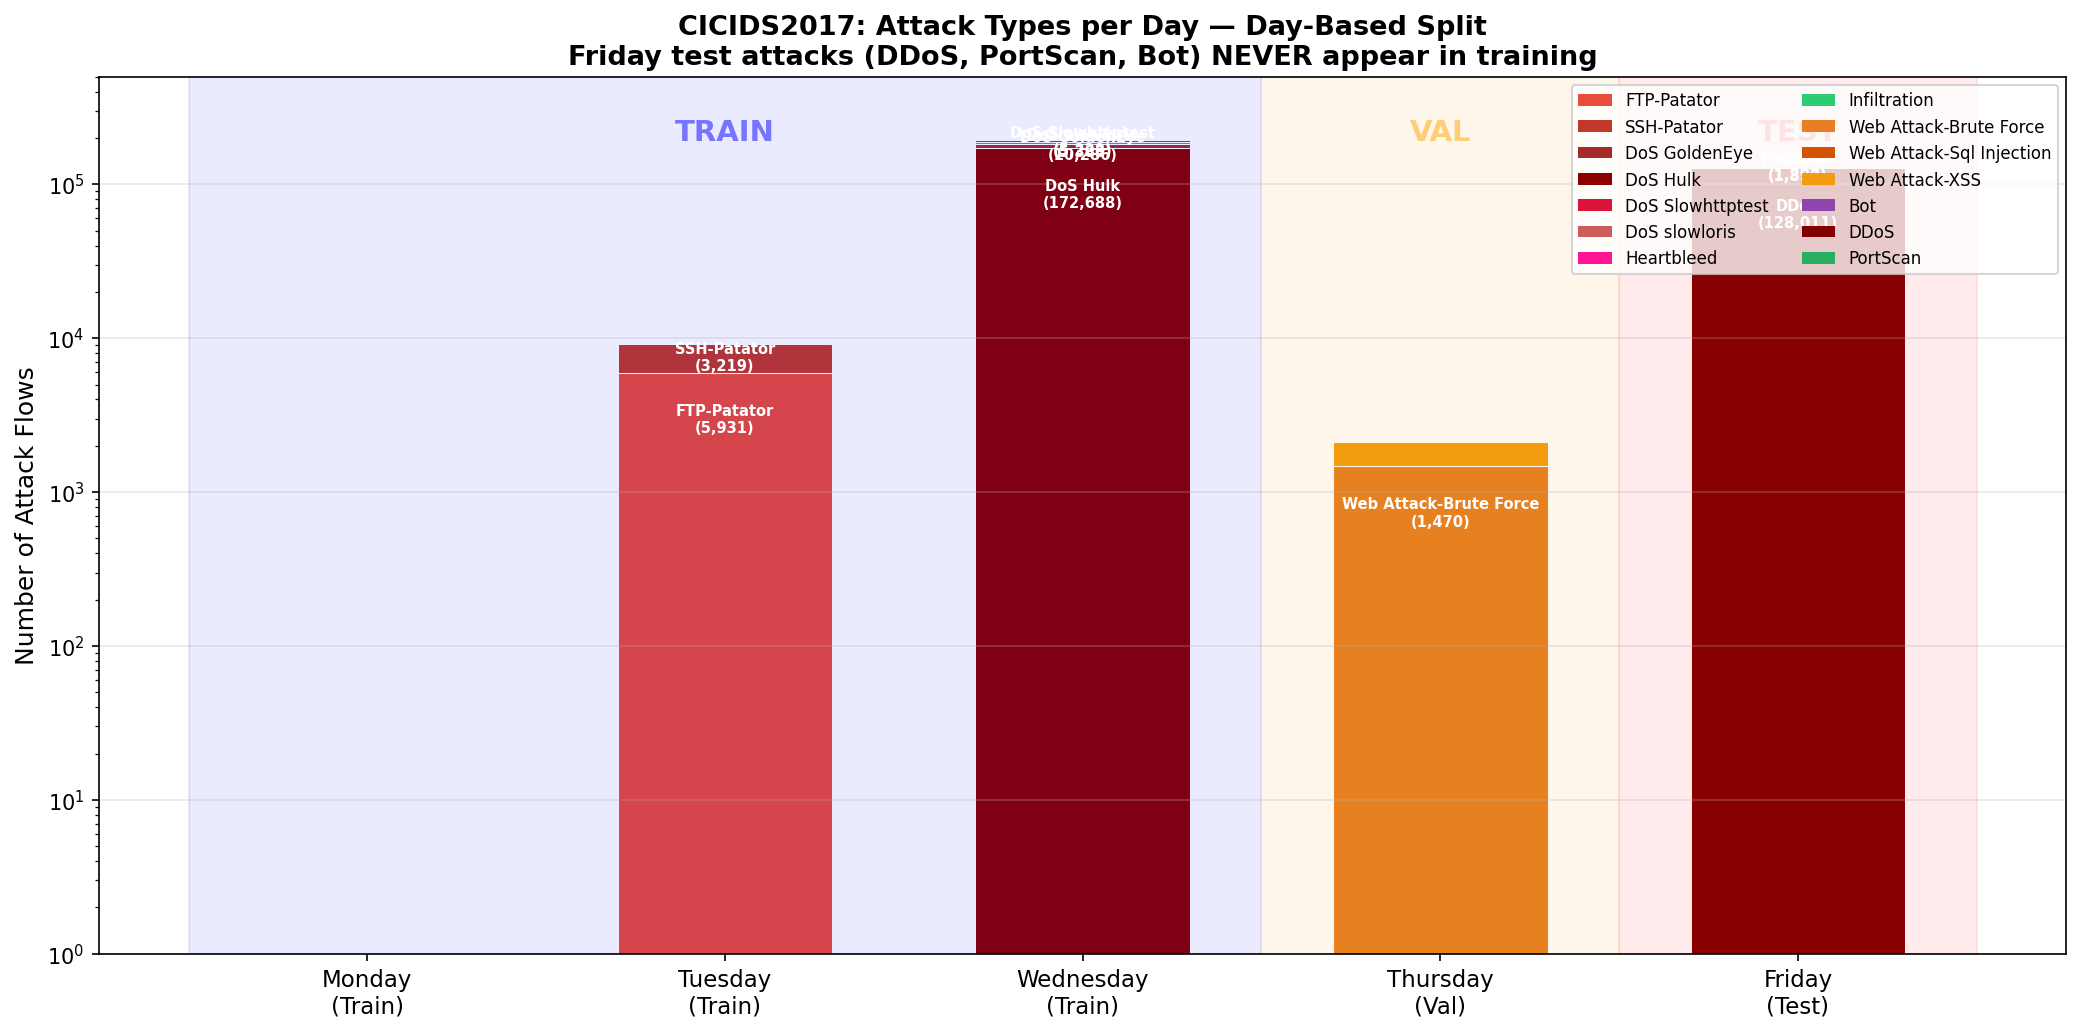
\includegraphics[width=0.95\textwidth]{day_attack_distribution.png}
    \caption{CICIDS2017 attack flows per day, coloured by attack type
    (log y-axis). Shaded regions mark the day-based train/val/test
    split.}
    \label{fig:day-attack-distribution}
\end{figure}

The dataset also exhibits extreme class imbalance: 85\% of flows are
benign, the most common attack class (DoS Hulk) has 172{,}688 flows, and
the rarest (Heartbleed) has only 11 --- a 220{,}000:1 ratio. We mitigate
imbalance with class-weighting strategies documented in
Chapter~\ref{ch:method} and use macro F1 as the headline metric.

\begin{figure}[H]
    \centering
    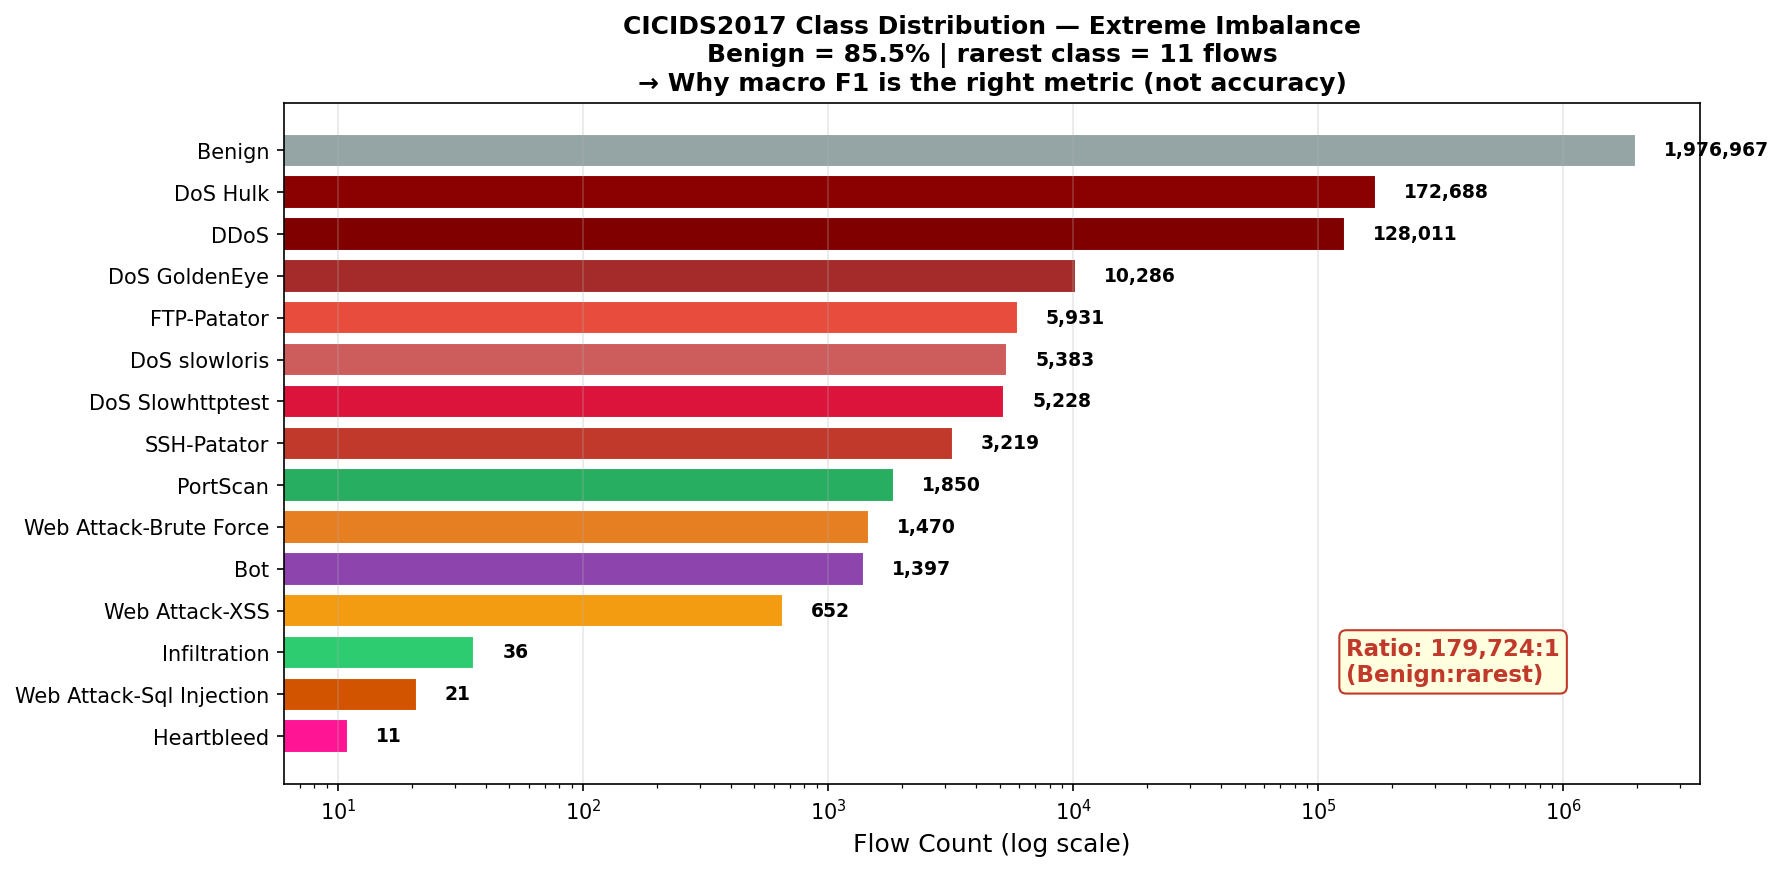
\includegraphics[width=0.8\textwidth]{class_imbalance.png}
    \caption{CICIDS2017 class distribution on a log scale.}
    \label{fig:class-imbalance}
\end{figure}

\section{UNSW-NB15 and the Need for Two Datasets}

UNSW-NB15~\cite{Moustafa2015,UNSW2015} is a 2.54-million-row capture from
the IXIA PerfectStorm platform with nine attack categories plus Normal.
We use the official train/test split with 175{,}341 test rows. UNSW
provides a useful cross-dataset comparison because it was generated by a
different team on a different testbed with a substantially different
attack catalogue, and the binary label distribution is more balanced
(attack rate $\approx$ 31\% versus CICIDS' 14\%).

A single-dataset claim is not really a claim about machine learning --- it
is a claim about that one dataset. By benchmarking on two independent
corpora we can distinguish robust patterns (which generalise) from
dataset artefacts (which do not). The rank-reversal between the two
datasets reported in Chapter~\ref{ch:crossdataset} is the main empirical
justification for the ``no universal winner'' conclusion.

\section{Data Cleaning Pipeline}
\label{sec:cleaning}

Raw CSVs from CIC contain duplicate rows, infinity values from divisions
by zero, and inconsistent column whitespace. The
\texttt{src/prepare\_data.py} module performs the following
deterministically: strip whitespace from column names; replace
$\pm\infty$ with NaN and drop NaN rows; deduplicate by hashing the full
feature-plus-label vector; add day-of-week and source-file columns; and
persist to a Parquet file of approximately 200~MB.

A key step is \textit{leakage filtering}. Engelen et al.~\cite{Engelen2021}
showed that several CICIDS2017 papers achieved their headline numbers
because the four rate features --- Flow Bytes/s, Flow Packets/s, Forward
and Backward Packets/s --- leak the label through their denominators. We
drop these four columns explicitly and the \texttt{src/leakage\_check.py}
module enforces their absence. Removing them alone lowers stratified
random-forest macro F1 by approximately four percentage points.
\label{sec:leakage}

\section{Train, Validation, and Test Splits}

Three split policies, each progressively more demanding. The
\textbf{stratified} split is a row-wise stratified partition preserving
class proportions across train, validation, and test partitions --- the
policy used in most prior work, producing the optimistic numbers. The
\textbf{day-based} split corresponds directly to the day-of-capture
column: train on Monday--Wednesday, validate on Thursday, test on Friday.
This is the realistic protocol for a deployed IDS. The
\textbf{leave-one-day-out (LODO)} split holds out one day for testing,
uses the remaining days for training and threshold-tuning validation, and
rotates through all five days. LODO is the strongest temporal
generalisation test because it exercises the model on five disjoint
held-out distributions.

A stratified split lets the model see Friday traffic during training,
memorise Friday-specific patterns, and report them as generalisation. A
day-based split forbids this, and the 0.4-macro-F1 gap between the two
policies is the memorisation tax. This pattern matches Pendlebury et
al.~\cite{Pendlebury2019}, who showed for malware classification that
random splits over-state deployment performance and proposed time-aware
evaluation as the default protocol --- a recommendation we adopt here.

\chapter{Experimental Methodology}
\label{ch:method}

\section{Models, Hyperparameters, and Evaluation Protocol}

Four supervised classifiers span the spectrum of complexity: logistic
regression (linear baseline), random forest (bagging ensemble), XGBoost
and LightGBM (gradient boosting). Two unsupervised baselines (Isolation
Forest, LOF) are run on the binary day task to compare against
label-free methods. Deep models are excluded because tree ensembles match
or exceed them on tabular flow features~\cite{Grinsztajn2022} and the
additional complexity would crowd out the adversarial and operational
analyses. Mirsky et al.~\cite{Mirsky2018} demonstrate that an
unsupervised autoencoder ensemble (Kitsune) can match supervised
baselines under streaming conditions; integrating their approach is left
to future work.

Hyperparameters were chosen from documented library defaults plus minor
coarse tuning on the stratified validation split. The full configuration
is in Appendix~A; the most relevant values are \texttt{n\_estimators=300}
for random forest, \texttt{max\_depth=8} and
\texttt{learning\_rate=0.1} for the gradient-boosting libraries, and a
\texttt{saga} solver with maximum 2000 iterations and balanced class
weights for logistic regression.

All metrics are reported on the held-out test split, never on validation.
Validation is used solely for threshold tuning via Youden's~J and early
stopping. Stratified results use the held-out stratified test partition;
day results use Friday; LODO results aggregate across the four
attack-bearing folds (Tuesday, Wednesday, Thursday, Friday; the Monday
fold is benign-only and contributes only an FPR measurement). UNSW
results use the official test split.

All headline binary day-split numbers carry 95\% percentile bootstrap
confidence intervals ($B = 1000$ resamples, seed 42). Pairwise model
comparisons use McNemar's test with Yates continuity correction;
every pairwise comparison is significant at $p < 10^{-4}$. Reproducibility:
every result comes from a single \texttt{make full} run that takes
45--60 minutes on a 2024 MacBook Pro M-series. The random seed is fixed
(\texttt{random\_state = 42}). Multi-threaded tree ensembles introduce
approximately 1\% F1 drift between runs because of non-deterministic
thread scheduling at leaf-split time.

\section{Design Decisions}
\label{sec:design}

Many of the most consequential choices in this project are not modelling
choices but framing choices. Table~\ref{tab:design-decisions} records the
choices made alongside the alternatives considered.

\begin{table}[H]
    \centering
    \caption{Design decisions: alternatives considered and rationale.}
    \label{tab:design-decisions}
    \footnotesize
    \begin{tabular}{p{2.6cm}p{4.0cm}p{2.6cm}p{4.4cm}}
        \toprule
        \textbf{Decision} & \textbf{Alternatives considered} & \textbf{Chosen} & \textbf{Rationale} \\
        \midrule
        Dataset & CICIDS2017, UNSW-NB15, CSE-CIC-IDS2018, NSL-KDD, KDDCup99 & CICIDS2017 + UNSW-NB15 & Modern benchmark plus independent testbed for cross-validation. \\
        \addlinespace
        Split protocol & Stratified random, K-fold CV, day-based, LODO & All three: stratified, day-based, LODO & Reporting all three exposes the gap between published-style and realistic protocols. \\
        \addlinespace
        Task framing & Multi-class, binary, hierarchical, anomaly only & Both multi-class and binary & Multi-class is standard; binary is deployable; comparing them is the headline finding. \\
        \addlinespace
        Models & LogReg, RF, XGBoost, LightGBM, SVM, MLP, LSTM, transformer & LogReg + RF + XGBoost + LightGBM & Tree ensembles dominate tabular benchmarks; linear baseline anchors comparison; deep models out of scope. \\
        \addlinespace
        Threshold method & 0.5, F1-optimal, Youden's J, FPR-constrained & Youden's J + FPR-constrained & Prevalence-invariant; matches real SOC alert-budget constraint. \\
        \addlinespace
        Metric & Accuracy, F1, macro F1, ROC-AUC, recall@FPR & Macro F1 + recall@FPR & Macro F1 weights classes equally; recall@FPR is deployment-relevant. \\
        \addlinespace
        Adversarial attack & FGSM, PGD, C\&W, greedy coordinate-ascent & Greedy coordinate-ascent (score-query black-box) & Tree ensembles non-differentiable; query-only attacks realistic for tabular IDS. \\
        \addlinespace
        Defence & Madry adv-training, randomisation, certified, ensembles & Naïve adversarial training & Simplest baseline; reporting that it fails is itself informative. \\
        \addlinespace
        Triage layer & Static MITRE, learned mapping & Static MITRE ATT\&CK & Realistic for BSc scope; learned mapping needs telemetry beyond available. \\
        \bottomrule
    \end{tabular}
\end{table}


\thesispart{Results}
\chapter{Multi-Class Classification Results}
\label{ch:multiclass}

\section{The Generalisation Collapse}

Table~\ref{tab:multiclass-headline} contains the central empirical claim
of the thesis. On the random stratified split, XGBoost achieves macro
F1 = 0.86 and random forest follows at 0.84. On the day-based split,
every tree ensemble collapses to a macro F1 in the 0.43--0.46 range. The
collapse is uniform across all three tree models, which differ by less
than 0.04 macro F1 on the day split. The reason: Friday's DDoS, PortScan,
and Bot classes never appear in Mon--Wed training, so the classifier
cannot output the correct label for those flows no matter how well it
is calibrated.

\begin{table}[H]
    \centering
    \caption{CICIDS2017 multi-class macro F1 by split policy.}
    \label{tab:multiclass-headline}
    \small
    \begin{tabular}{lccc}
        \toprule
        \textbf{Model} & \textbf{Stratified} & \textbf{Day-based} & \textbf{$\Delta$} \\
        \midrule
        LogReg & 0.266 & 0.429 & +0.163 \\
        Random Forest & 0.845 & 0.438 & $-$0.407 \\
        XGBoost & 0.863 & 0.440 & $-$0.423 \\
        LightGBM & 0.300 & 0.463 & +0.163 \\
        \bottomrule
    \end{tabular}
\end{table}

\interpretation{The 0.4-point drop for tree ensembles between split
policies is the single largest signal in this thesis. The published
numbers reflect in-distribution memorisation, not deployment readiness.}

\begin{figure}[H]
    \centering
    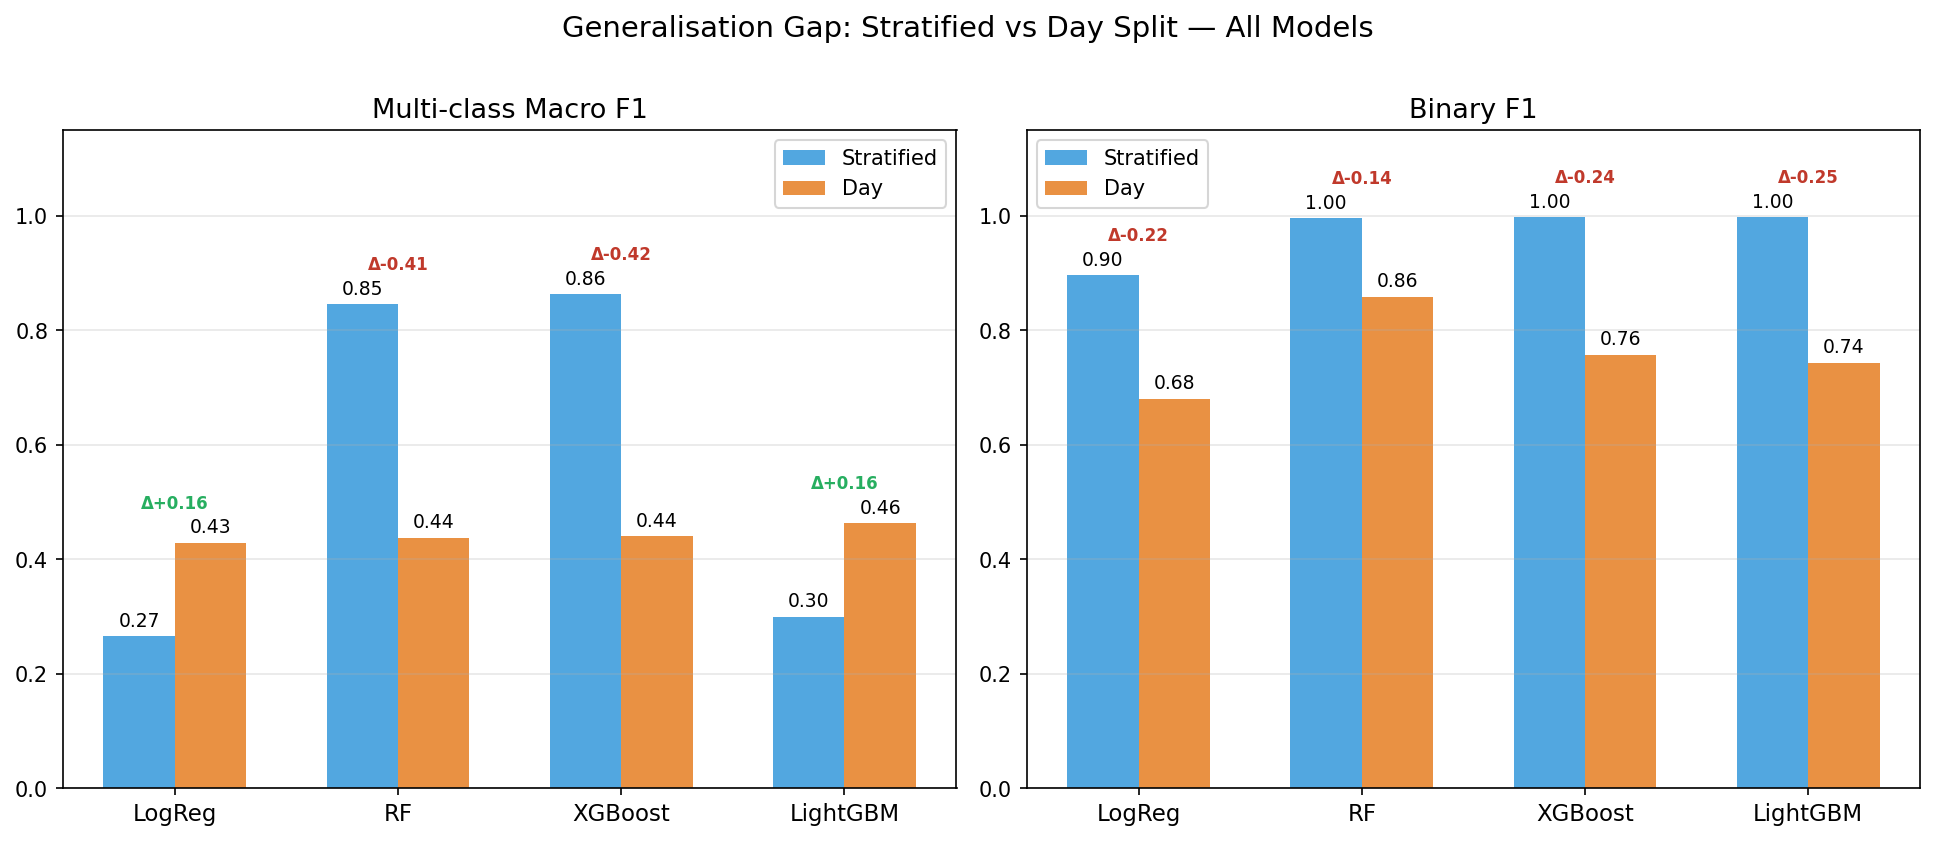
\includegraphics[width=0.95\textwidth]{generalisation_gap_all_models.png}
    \caption{Stratified versus day-split macro F1 across all four models.
    Blue bars are stratified (published-style); red bars are day-based
    (deployment-style). Every tree ensemble loses around 0.4 macro F1.}
    \label{fig:gen-gap}
\end{figure}

Logistic regression behaves differently: its macro F1 actually
\textit{improves} from 0.27 stratified to 0.43 on the day split. Its
stratified score was already low because it cannot capture the non-linear
class boundaries that tree models exploit. On the day split, the unseen
classes hurt all models equally, but the tree models also lose the
spurious correlations they had memorised, while logistic regression had
not learned those correlations to begin with.

\section{Why Multi-Class Collapses: Confusion Analysis}

The day-split confusion matrix shows the failure mode. Friday DDoS flows
are predominantly predicted as DoS Hulk, the closest seen class in
feature space. PortScan splits between DoS Hulk and Benign. Bot is
mostly predicted as Benign, because without seeing C2 traffic in
training the model cannot distinguish a periodic beacon from background
process traffic. Every Friday error is structural --- a consequence of a
label not existing in training rather than a tunable model failure ---
and it cannot be addressed by additional training on the same days.

\begin{figure}[H]
    \centering
    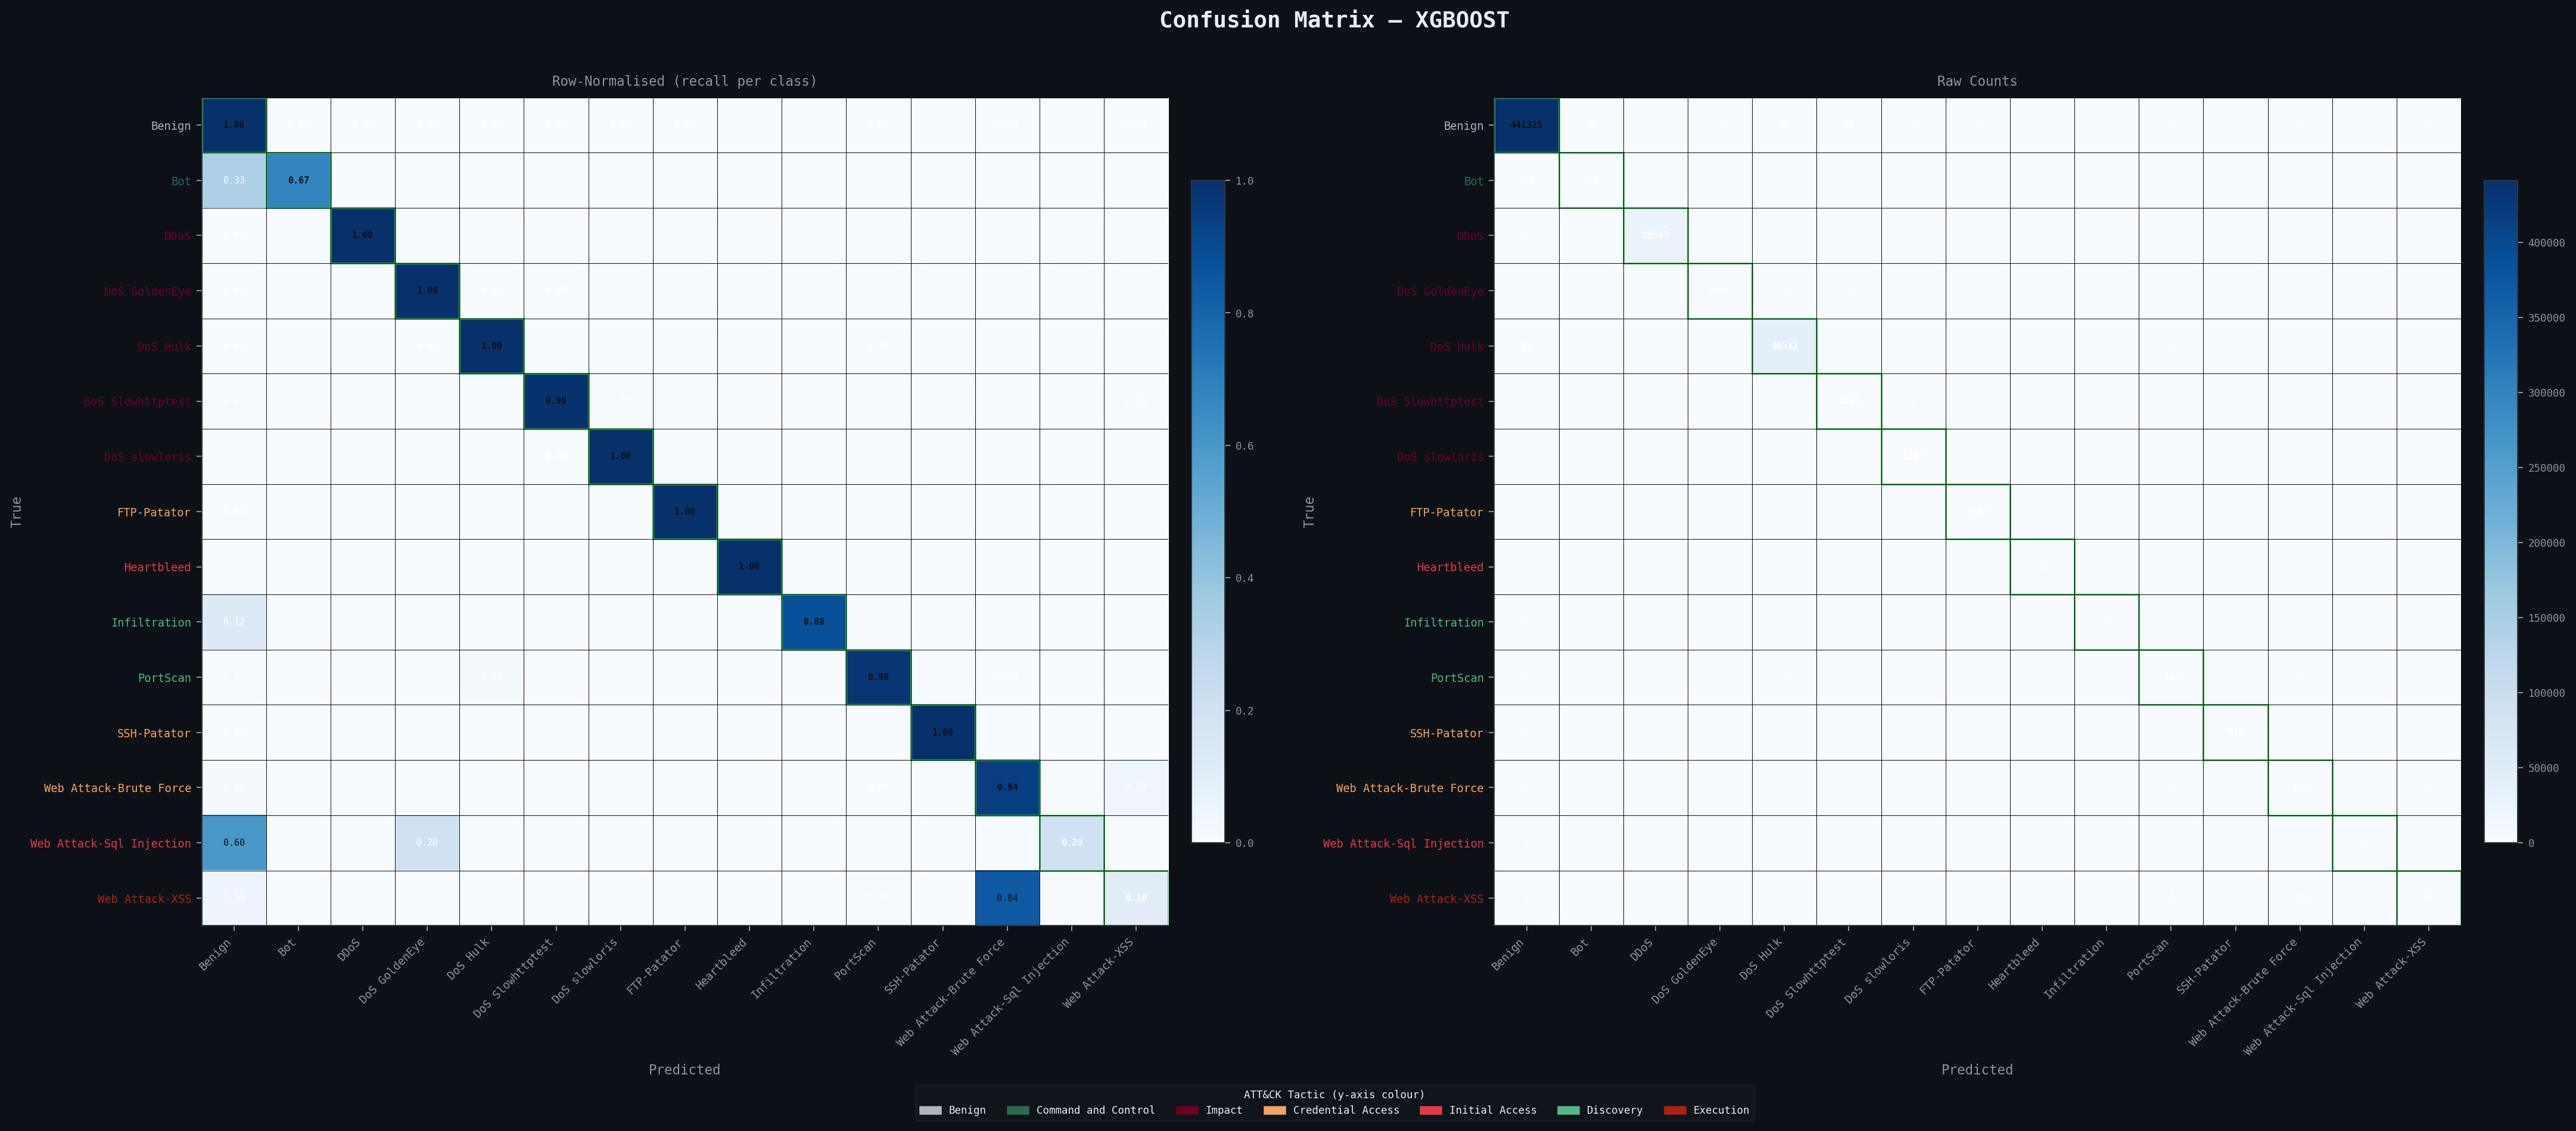
\includegraphics[width=0.95\textwidth]{confusion_matrix.png}
    \caption{Confusion matrices: stratified split (left) versus day split
    (right) for the best multi-class model. On stratified the diagonal
    is bright everywhere; on day the Friday rows (DDoS, PortScan, Bot)
    are entirely off-diagonal.}
    \label{fig:cm}
\end{figure}

Per-class F1 on the day split is exactly 0.0 for DDoS, PortScan, and Bot
across all four models. The 0.44 macro F1 reported above comes entirely
from the Benign class and the few attack classes that overlap between
Mon--Wed training and Thu--Fri evaluation.

\section{Feature Importance and Per-Instance Interpretability}

The structural failure of multi-class classification on the day split
does not invalidate everything that has been learned. The features that
drive the in-distribution model tell us which flow statistics carry the
most discriminative power and therefore which features an attacker would
need to manipulate to evade detection. The XGBoost gain-based importance
ranks Backward Packet Length Std, Idle Mean, Forward Active Data Packets,
and Backward Packet Length Mean as the top four features. Server-side
response statistics carry most of the discriminative power. A
random-forest permutation-importance check produces a similar ranking,
which gives us confidence that the signal is real rather than a quirk
of the gain calculation.

\begin{figure}[H]
    \centering
    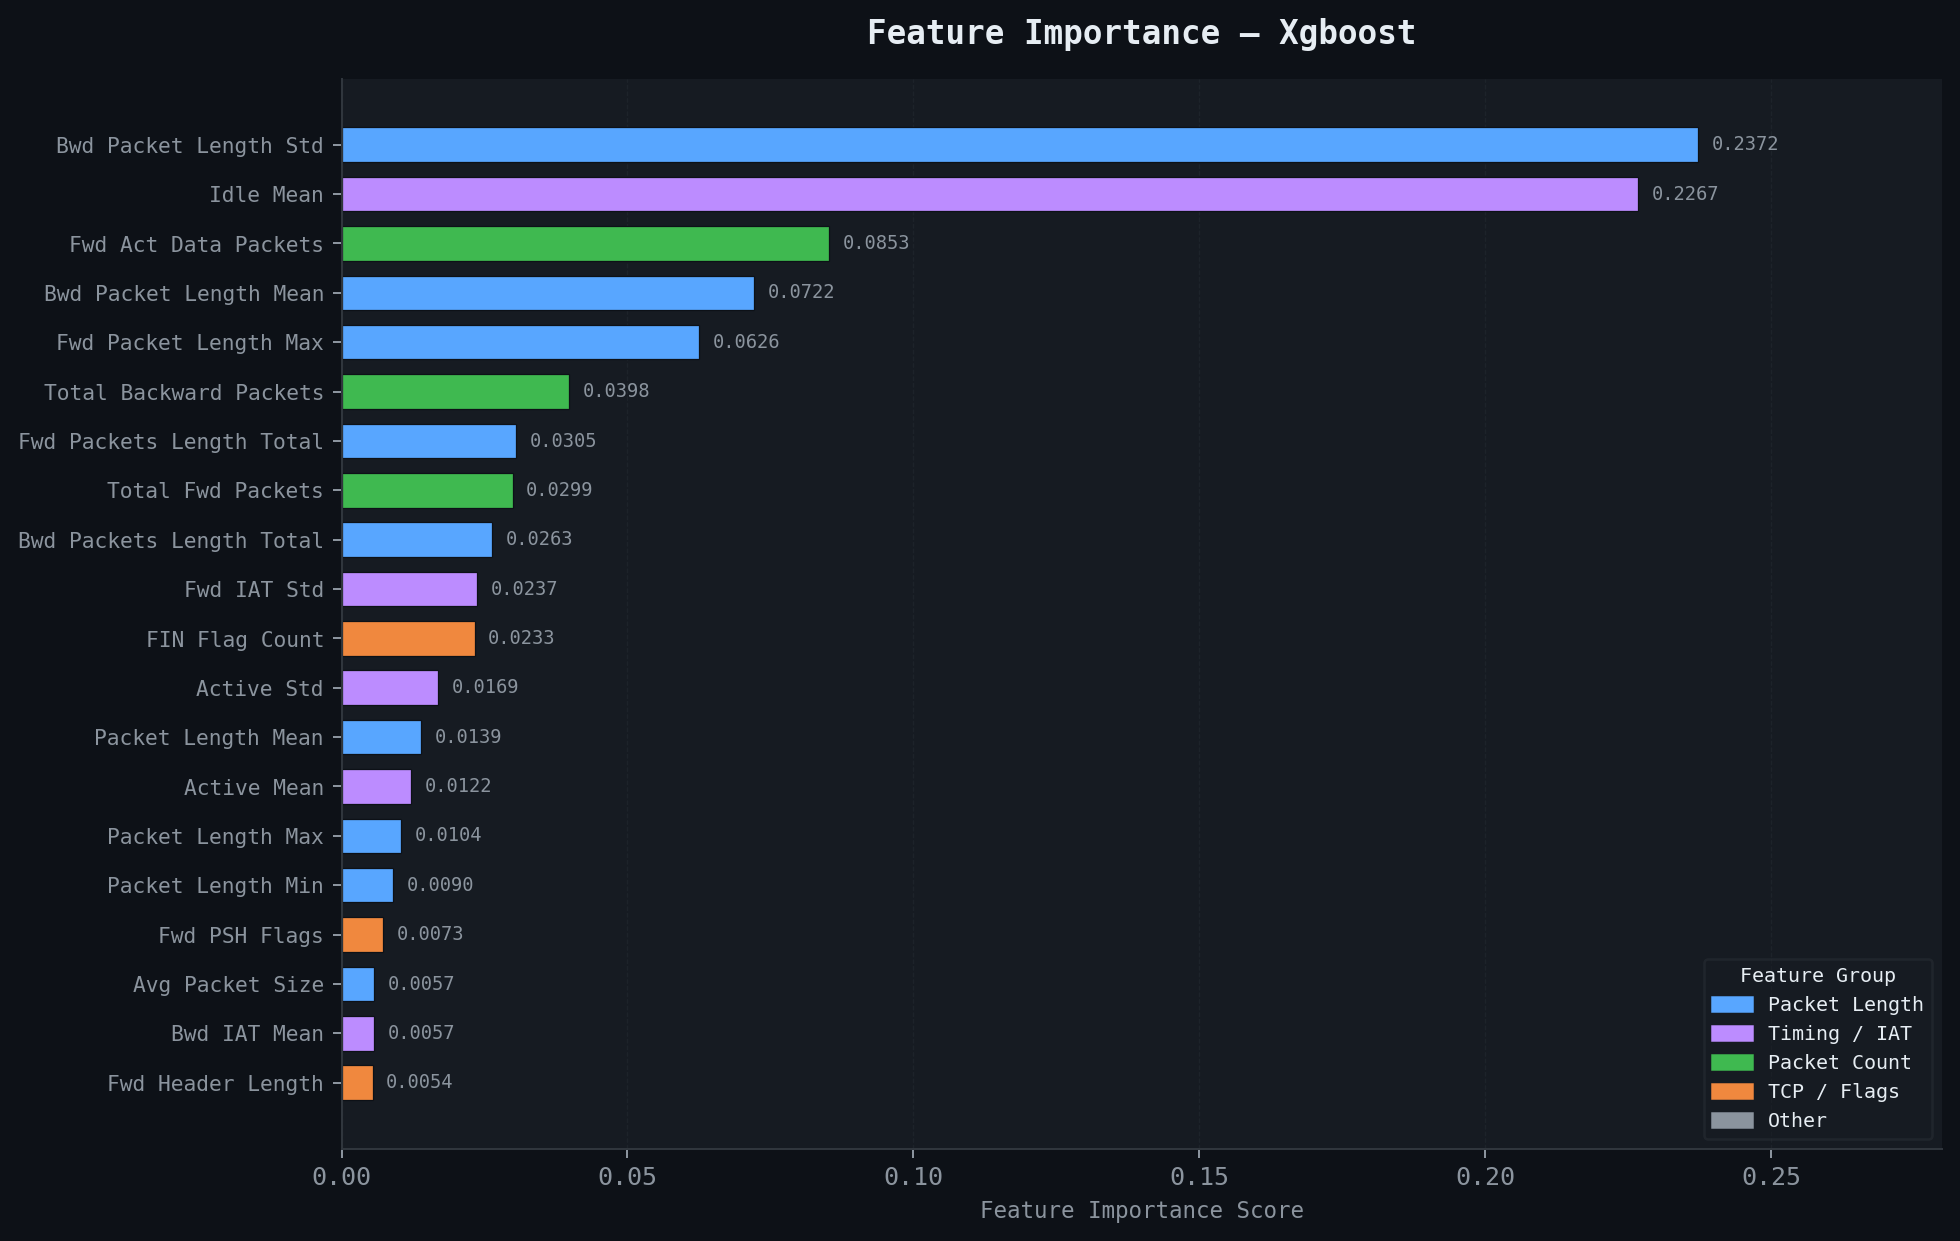
\includegraphics[width=0.8\textwidth]{feature_importance_xgboost.png}
    \caption{XGBoost gain-based feature importance (top features).}
    \label{fig:fi-xgb}
\end{figure}

For per-instance interpretability we use SHAP. The SHAP summary plot for
the binary random-forest detector shows that small Flow IAT Min values
push predictions strongly toward the attack class --- exactly the pattern
an attacker would observe and exploit, as confirmed in
Chapter~\ref{ch:adversarial}.

\begin{figure}[H]
    \centering
    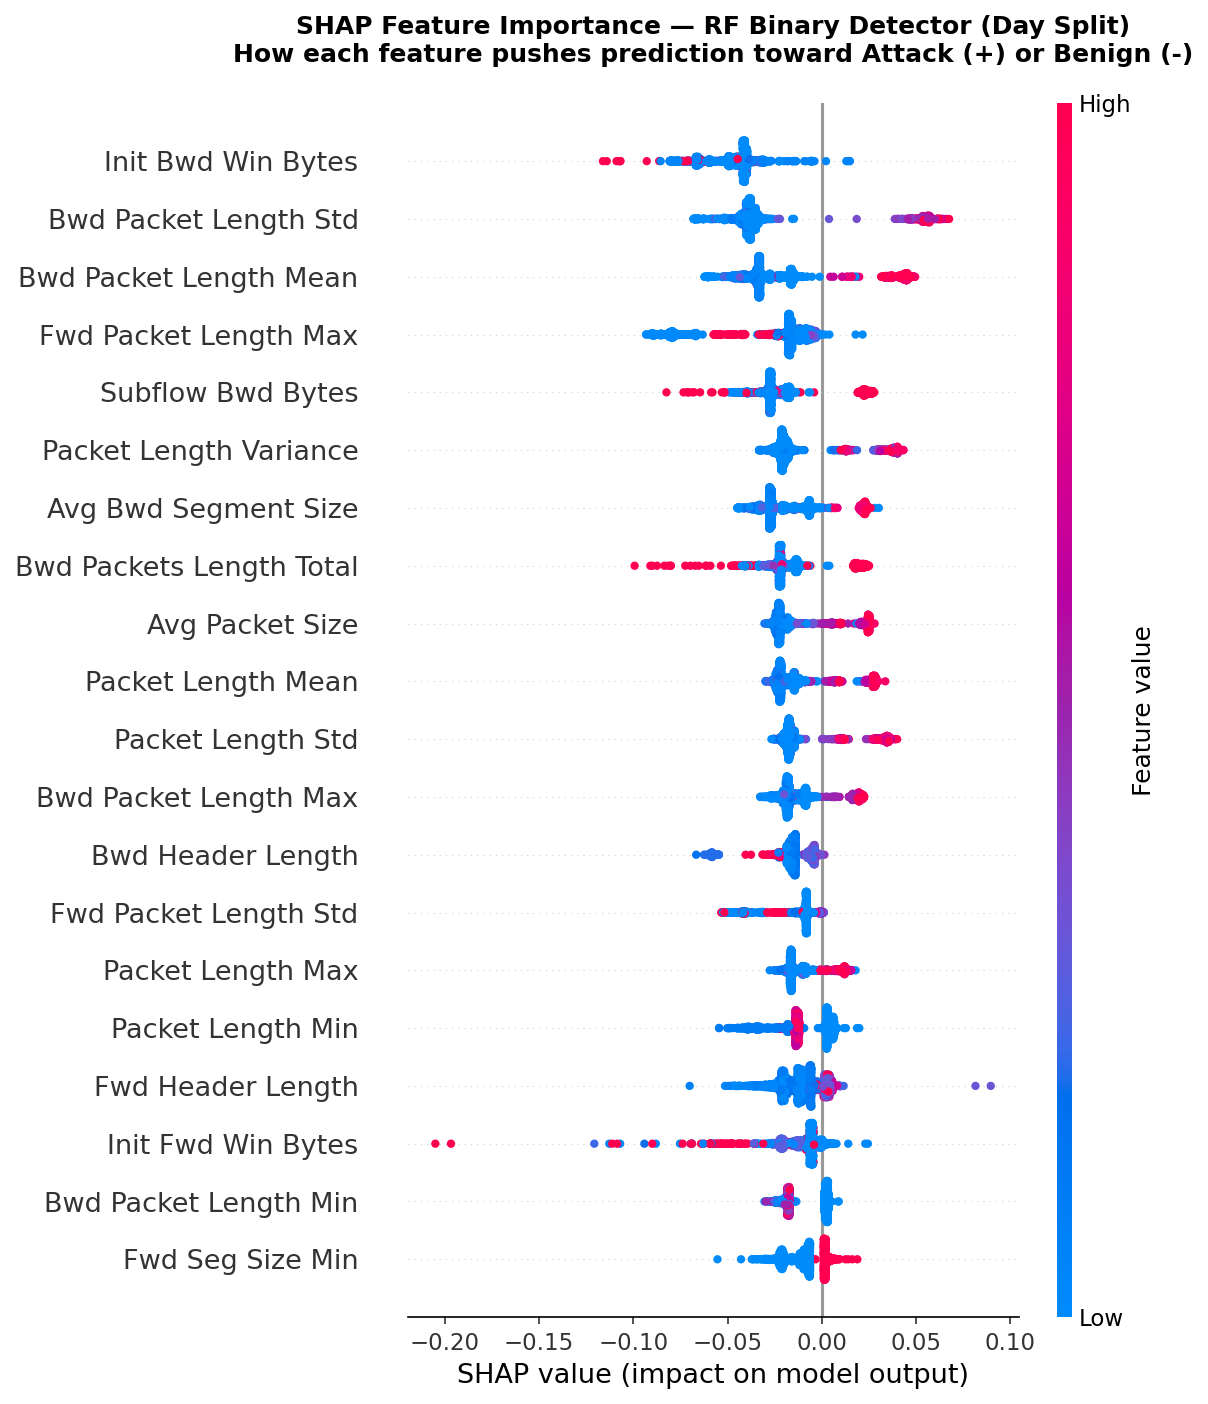
\includegraphics[width=0.7\textwidth]{shap_summary_rf_binary.png}
    \caption{SHAP summary plot for the binary RF detector. Each dot is one
    flow; colour is feature value; position is the SHAP value.}
    \label{fig:shap-summary}
\end{figure}

\chapter{Binary Detection Results}
\label{ch:binary}

\section{Headline Numbers}

Reframing the task as ``benign versus any-attack'' recovers most of the
performance lost in the multi-class collapse. Random forest reaches
F1 = 0.86 on the day split, within 0.14 of its stratified score of 0.996.
XGBoost and LightGBM trail random forest on the day split (F1
0.74--0.76) despite higher stratified scores, because their decision
boundaries over-fit the Mon--Wed attacks.

\begin{table}[H]
    \centering
    \caption{CICIDS2017 binary F1 at the Youden-J threshold.}
    \label{tab:binary-headline}
    \small
    \begin{tabular}{lcccc}
        \toprule
        \textbf{Model} & \textbf{Stratified F1} & \textbf{Day F1} & \textbf{Day Threshold} & \textbf{Day ROC-AUC} \\
        \midrule
        LogReg & 0.896 & 0.681 & 0.0627 & 0.981 \\
        Random Forest & 0.996 & \textbf{0.859} & 0.0090 & 0.940 \\
        XGBoost & 0.997 & 0.757 & 0.000323 & 0.972 \\
        LightGBM & 0.998 & 0.744 & 0.000178 & 0.957 \\
        \bottomrule
    \end{tabular}
\end{table}

\interpretation{The thresholds in column four are striking: tree
ensembles need to operate at probabilities below $10^{-3}$ on the day
split. Reporting F1 at the canonical 0.5 threshold would yield F1
$\approx 0.007$ for XGBoost. Threshold transfer is not optional --- it
is a first-class deployment concern.}

\section{Operating Points and Calibration}
\label{sec:operating-points}

For deployment, the question is not which threshold maximises F1 but
which threshold meets a fixed false-positive budget. A SOC can absorb a
finite number of false alerts per analyst per shift, so the
operationally relevant metric is recall at a fixed FPR.
Table~\ref{tab:operating-points} reports recall at three FPR budgets
(0.01\%, 0.1\%, 1\%) per model on the binary day split, alongside the
Expected Calibration Error (ECE) that explains the pattern.

\begin{table}[H]
    \centering
    \caption{Recall at fixed FPR budgets on the binary day split
    ($n = 516{,}643$, attack rate $0.2541$). ECE is the Expected
    Calibration Error with 15 equal-width bins; lower is better.}
    \label{tab:operating-points}
    \small
    \begin{tabular}{lcccc}
        \toprule
        \textbf{Model} & \textbf{ECE $\downarrow$} & \textbf{Recall @ 0.01\% FPR} & \textbf{Recall @ 0.1\% FPR} & \textbf{Recall @ 1\% FPR} \\
        \midrule
        LogReg & 0.073 & 0.393 & 0.394 & 0.605 \\
        Random Forest & 0.178 & 0.000 & \textbf{0.621} & 0.634 \\
        XGBoost & 0.252 & 0.001 & 0.031 & \textbf{0.637} \\
        LightGBM & 0.249 & 0.001 & 0.461 & 0.620 \\
        \bottomrule
    \end{tabular}
\end{table}

A 0.1\% FPR budget on a two-million-flow day produces around 2{,}000
false alerts, which is the regime where a small SOC can absorb the alert
volume without burning analyst hours; the 1\% budget is closer to a
large enterprise with more analysts on the queue. Random forest
dominates the strict end of the curve and XGBoost catches up only as the
FPR budget loosens.

\begin{figure}[H]
    \centering
    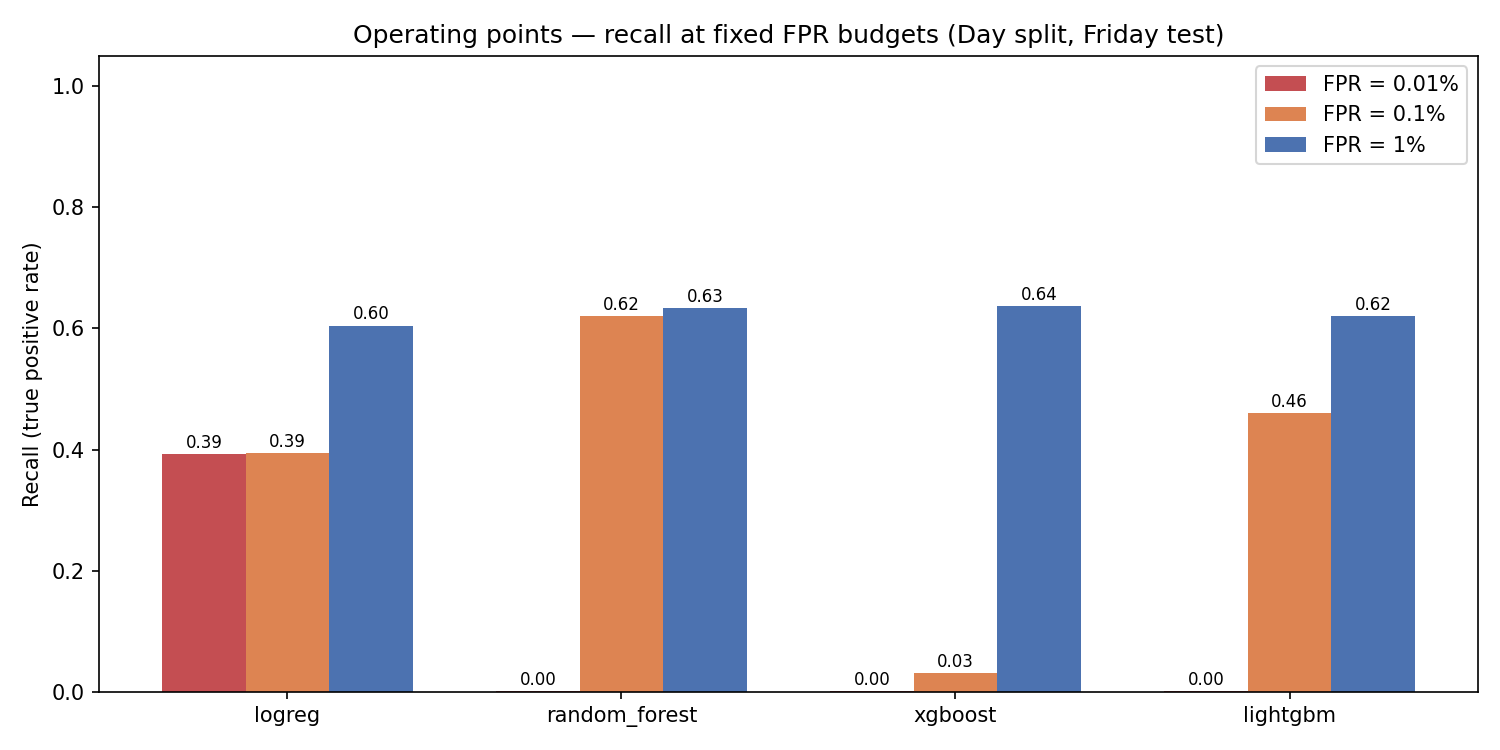
\includegraphics[width=0.8\textwidth]{operating_points.png}
    \caption{Recall at fixed FPR budgets per model on the binary day
    split. At a 1\% FPR budget all four models recover similar recall
    (60--64\%); at the tighter 0.1\% FPR budget, random forest still
    catches 62\% of attacks while XGBoost drops to 3\%.}
    \label{fig:op-points}
\end{figure}

Calibration explains why the operating-point picture varies so much
between models. Logistic regression on the day split is nearly perfectly
calibrated (ECE = 0.073); tree ensembles are markedly less so (RF 0.18,
XGB and LGB 0.25). Poor calibration is exactly why the canonical 0.5
threshold fails for tree ensembles under temporal shift, and why
Youden's J on validation is needed to recover sensible operating points.

\section{Statistical Significance}
\label{sec:mcnemar}

Two statistical tests support the model ranking. McNemar's test with
Yates continuity correction on every pair of models on the binary
day-split test set rejects the null of equal error rates at $p < 10^{-4}$
for all six pairs, including the closest (XGBoost versus LightGBM,
$\chi^2 = 520.6$). Bootstrap 95\% confidence intervals (with
$B = 1000$ resamples on $n = 516{,}643$ test flows) are correspondingly
narrow, typically about $\pm 0.001$ on F1, and confirm the same ordering.
Random forest has the highest F1 with non-overlapping precision/recall
confidence intervals against all other models.

\chapter{Leave-One-Day-Out Cross-Validation}
\label{ch:lodo}

The day-based split tests one specific scenario --- train on
Monday-to-Wednesday, test on Friday --- and is therefore vulnerable to the
criticism that the result might be a quirk of that particular split.
Leave-one-day-out (LODO) cross-validation answers this concern by
holding out one day for testing, training on the remaining days with
one as inner-validation for threshold tuning, then rotating through
all five days. The Monday fold is benign-only and so reports only an FPR
measurement; the remaining four folds (Tuesday--Friday) bear attacks and
contribute to F1, ROC-AUC, and PR-AUC. The mean and standard deviation
across these four attack-bearing folds is the headline LODO result.

\begin{table}[H]
    \centering
    \caption{LODO mean $\pm$ std across the 4 attack-bearing folds (Tuesday--Friday).}
    \label{tab:lodo}
    \small
    \begin{tabular}{lcccc}
        \toprule
        \textbf{Model} & \textbf{ROC-AUC} & \textbf{PR-AUC} & \textbf{F1} & \textbf{FPR} \\
        \midrule
        LogReg & $0.630 \pm 0.374$ & $0.299 \pm 0.439$ & $0.293 \pm 0.347$ & $0.292 \pm 0.412$ \\
        Random Forest & $\mathbf{0.926 \pm 0.053}$ & $0.632 \pm 0.354$ & $\mathbf{0.549 \pm 0.366}$ & $\mathbf{0.065 \pm 0.050}$ \\
        XGBoost & $0.921 \pm 0.086$ & $0.675 \pm 0.374$ & $0.437 \pm 0.353$ & $0.118 \pm 0.080$ \\
        LightGBM & $0.838 \pm 0.212$ & $0.580 \pm 0.363$ & $0.340 \pm 0.303$ & $0.173 \pm 0.102$ \\
        \bottomrule
    \end{tabular}
\end{table}

Random forest dominates on stability: ROC-AUC $= 0.926 \pm 0.053$ across
folds is the lowest standard deviation by a clear margin (XGBoost
$\pm 0.086$, LightGBM $\pm 0.212$, logistic regression $\pm 0.374$). The
false-positive rate is also the lowest at $6.5\% \pm 5.0\%$. XGBoost
matches RF on AUC but its threshold transfers poorly between days, which
is why its F1 spread ($0.437 \pm 0.353$) is much wider than random
forest's ($0.549 \pm 0.366$). LightGBM and logistic regression degrade
more sharply still.

\begin{figure}[H]
    \centering
    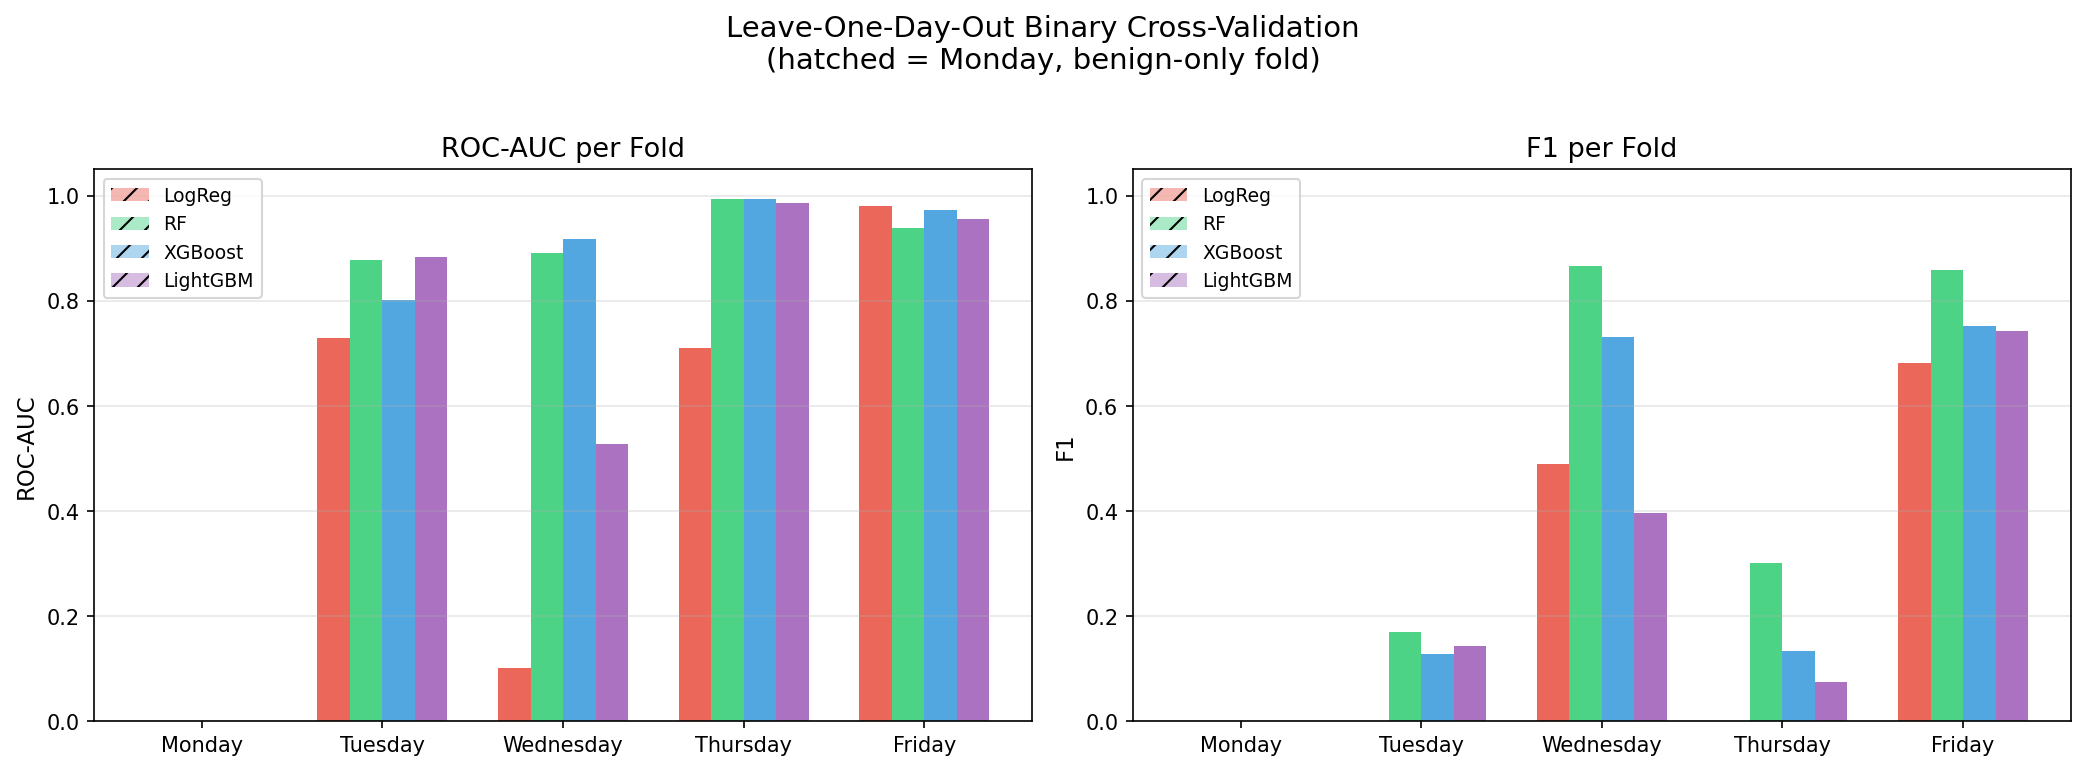
\includegraphics[width=0.95\textwidth]{lodo_folds.png}
    \caption{Per-fold ROC-AUC and F1 for all four models across the four
    attack-bearing days. Random forest's bars cluster tightly around 0.93
    ROC-AUC; LightGBM scatters from 0.53 to 0.99.}
    \label{fig:lodo}
\end{figure}

The LODO result strengthens the empirical case for random forest as the
deployable model. A single split gives one number; LODO gives a
distribution. A model with mean ROC-AUC $= 0.926$ and standard deviation
of only $0.053$ across genuinely disjoint test scenarios is more
trustworthy in production than a model that hits 0.99 on one split and
0.53 on another. The operational lesson is that stability across days is
a stronger generalisation claim than any single fold's headline F1.

\chapter{Cross-Dataset Validation on UNSW-NB15}
\label{ch:crossdataset}

The CICIDS2017 results so far are internally consistent: random forest
is the most temporally robust binary detector, and the binary task
survives temporal shift while the multi-class task does not. The
question this chapter addresses is whether those conclusions transfer
to a different dataset --- specifically, UNSW-NB15, generated by a
different team using a different testbed and a substantially different
attack catalogue.

Table~\ref{tab:unsw} reports UNSW-NB15 macro F1 for the multi-class task
and F1 for the binary task using the official train/test split
(175{,}341 test rows). The model ranking flips in the multi-class
setting: LightGBM leads at 0.548, XGBoost trails at 0.522, random forest
is third at 0.479, and logistic regression is last at 0.404. The binary
setting is much more uniform, with all three tree models clustered
around F1 $\approx 0.92$ and ROC-AUC $\approx 0.986$.

\begin{table}[H]
    \centering
    \caption{UNSW-NB15 macro F1 (multi-class) and F1 (binary) using the
    official train/test split.}
    \label{tab:unsw}
    \small
    \begin{tabular}{lccc}
        \toprule
        \textbf{Model} & \textbf{Multi-class F1} & \textbf{Binary F1} & \textbf{Binary ROC-AUC} \\
        \midrule
        LogReg & 0.404 & 0.888 & 0.976 \\
        Random Forest & 0.479 & 0.921 & 0.986 \\
        XGBoost & 0.522 & 0.919 & 0.986 \\
        LightGBM & \textbf{0.548} & 0.921 & 0.986 \\
        \bottomrule
    \end{tabular}
\end{table}

\begin{figure}[H]
    \centering
    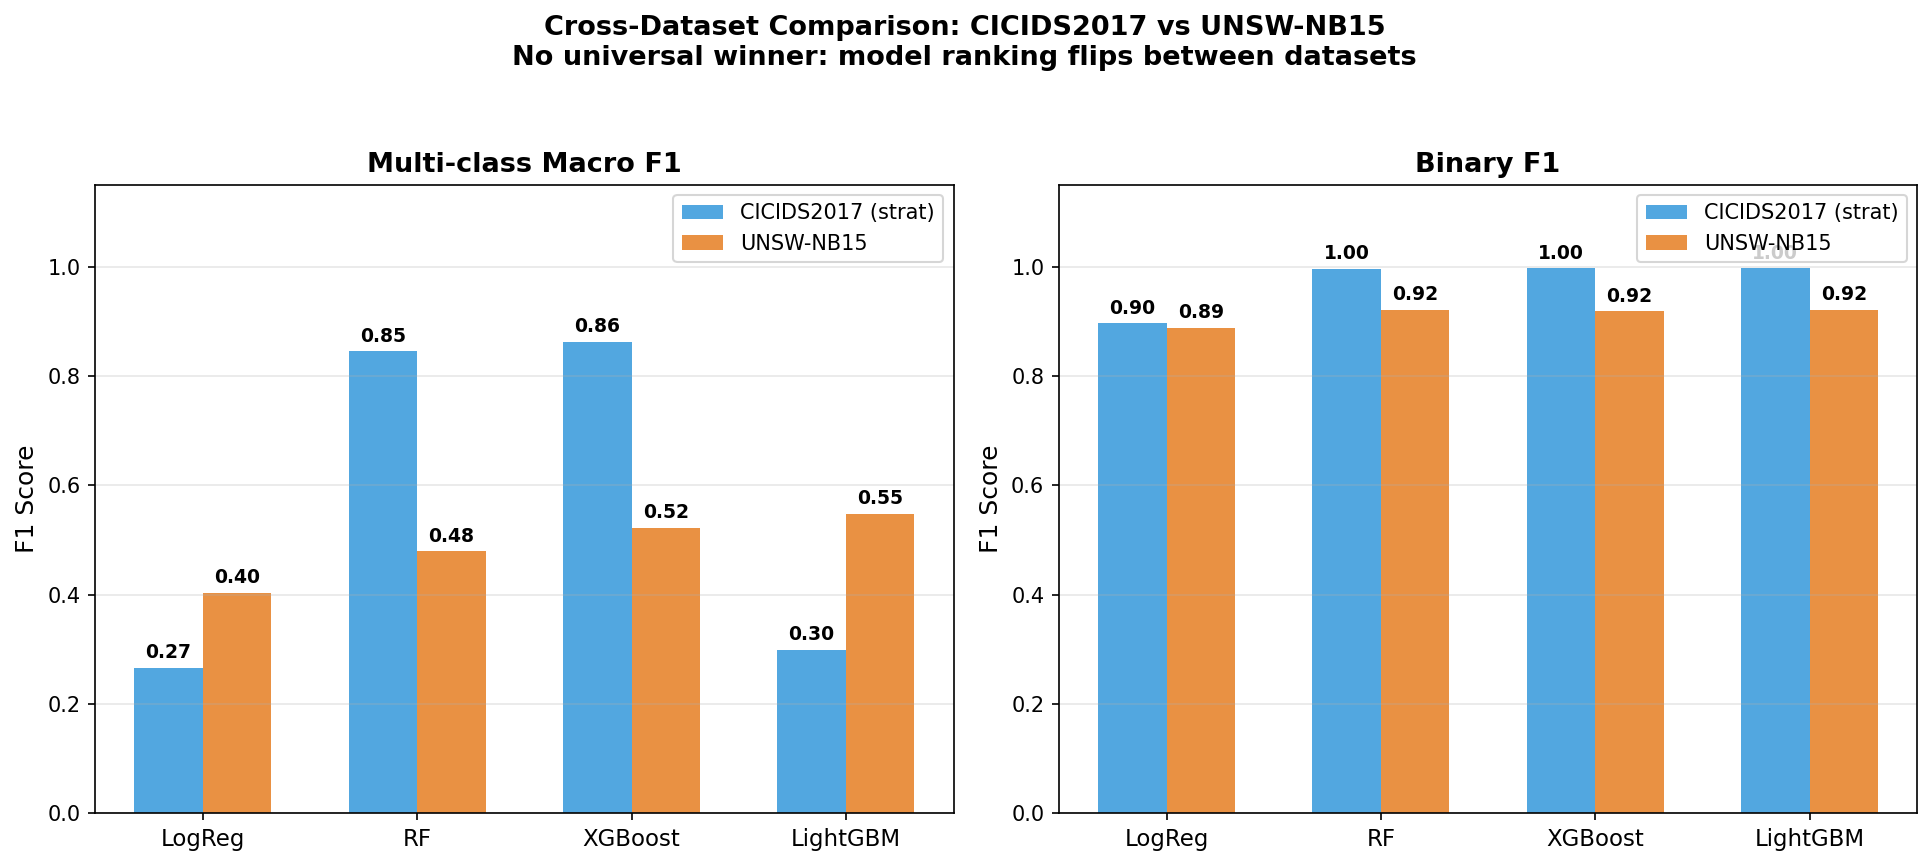
\includegraphics[width=0.95\textwidth]{cross_dataset_comparison.png}
    \caption{Model performance side-by-side on CICIDS2017 versus
    UNSW-NB15. The model ranking flips between datasets in the
    multi-class setting --- XGBoost wins on CICIDS multi-class but
    LightGBM wins on UNSW.}
    \label{fig:cross-comparison}
\end{figure}

The rank reversal between datasets is the most important cross-dataset
finding. No single tree ensemble dominates universally, and the headline
choice of ``best model'' depends on which dataset the benchmark is run
on. Practitioners who deploy a model based on a single-dataset result
should be aware that the same model may perform poorly on traffic from a
different testbed, and that validation on at least two independent
datasets is a minimum quality bar before claiming a universal winner.

The mechanism behind the rank reversal is feature-distribution
mismatch. On CICIDS, the top-ranked features for random forest are
inter-arrival-time statistics, because CICIDS attacks differ most from
benign traffic in their timing structure. On UNSW, the top-ranked
features are protocol and service categorical features
(\texttt{service\_dns}, \texttt{state\_INT}, \texttt{ct\_dst\_sport\_ltm}),
because UNSW attacks differ most from benign traffic in which services
they target and how connection states evolve. A model that best exploits
the dominant feature family on one dataset is not the best on the other.

\chapter{Adversarial Robustness}
\label{ch:adversarial}

The previous chapters established that the binary random forest is the
most temporally robust flow-based detector among the four models. This
chapter asks a different question: how robust is that detector against
an attacker who knows it is there and tries to evade it? The answer is
unsatisfying. Even a simple, score-query black-box greedy attack flips
a substantial fraction of attack flows to benign within a small
perturbation budget, the resulting adversarial flows transfer almost
completely to the second-best model, and a naïve adversarial-training
defence makes the situation worse rather than better.

\section{Threat Model and Attack}

The threat model assumes a \emph{score-query black-box} attacker: the
adversary can request the model's predicted probability for any input
flow but has no access to gradients, model parameters, or training data,
and we further assume no rate limit on queries. This is the realistic
capability for an external attacker that interacts with a deployed IDS
only through the network traffic it generates. The adversary's goal is
\textit{evasion}: flipping a true-attack flow to be classified as
benign, while keeping the perturbation small enough that the resulting
flow is still operationally plausible. Of the 73 features that survive
leakage filtering, only 19 are perturbable in practice --- timing
statistics, packet lengths, packet counts, and flow duration. The
remaining 54 features are determined by the underlying network stack
and cannot be freely manipulated by an application-level attacker.

The score-query black-box assumption is realistic in the sense documented
by Apruzzese et al.~\cite{Apruzzese2023}: real-world attackers ``do not
compute gradients'' against deployed IDS, so adversarial-ML evaluations
that assume full white-box gradient access overstate the threat. A more
sophisticated robustness audit would use AutoAttack-style
ensembles~\cite{Croce2020}, but greedy coordinate-ascent is a fair upper
bound on what a black-box adversary can achieve under these constraints.

The attack itself is greedy coordinate-ascent. At each iteration, the
attacker tries six candidate step magnitudes in each of the 19
perturbable features and keeps the perturbation that most reduces the
model's predicted attack probability. The procedure runs for up to 15
iterations per flow, and the perturbation is bounded in the $L^\infty$
norm by a budget $\varepsilon$ measured in units of benign-feature
standard deviations $\sigma$.

A second important caveat: the perturbations crafted here live in
\textit{feature} space, not in \textit{packet} space. Pierazzi et
al.~\cite{Pierazzi2020} formalised this distinction as the
``problem-space'' versus ``feature-space'' gap: a flow vector that the
attack algorithm produces may not correspond to any realisable packet
sequence that the attacker can transmit on the wire. This thesis stays
in feature space; bridging the gap to genuine packet-level adversarial
flows is open work.

\section{Evasion, Transferability, and the Failure of Naïve Defence}

Two related but distinct quantities are reported. The \emph{evasion
rate} of 0.244 is measured on a sample of 500 correctly-classified
attack flows when the greedy attack is allowed to run until its
perturbation is minimised or its iteration budget is exhausted; the
median $L^\infty$ distance needed to flip a prediction is $0.250\sigma$.
The \emph{robust accuracy} curve in Table~\ref{tab:robust-acc} measures
a different quantity: the fraction of attack flows whose prediction
survives when the perturbation is hard-bounded at a fixed $\varepsilon$.
At $\varepsilon = 0.25\sigma$, robust accuracy is 0.786, meaning that
21.4\% of attack flows lose their attack label under a $0.25\sigma$
budget. The 24.4\% headline evasion rate is the looser, unbounded
version of the same effect. The curve flattens quickly after
$\varepsilon = 0.5\sigma$: most flows that can be flipped at all are
already flipped at the smallest budget.

\begin{table}[H]
    \centering
    \caption{Robust accuracy: fraction of attack flows surviving evasion at increasing budgets.}
    \label{tab:robust-acc}
    \small
    \begin{tabular}{lcccc}
        \toprule
        \textbf{Model} & \textbf{$\varepsilon = 0.25\sigma$} & \textbf{$\varepsilon = 0.5\sigma$} & \textbf{$\varepsilon = 1.0\sigma$} & \textbf{$\varepsilon = 2.0\sigma$} \\
        \midrule
        Undefended RF & 0.786 & 0.772 & 0.756 & 0.756 \\
        Adv-trained RF & 0.736 & 0.732 & 0.732 & 0.732 \\
        \bottomrule
    \end{tabular}
\end{table}

\begin{figure}[H]
    \centering
    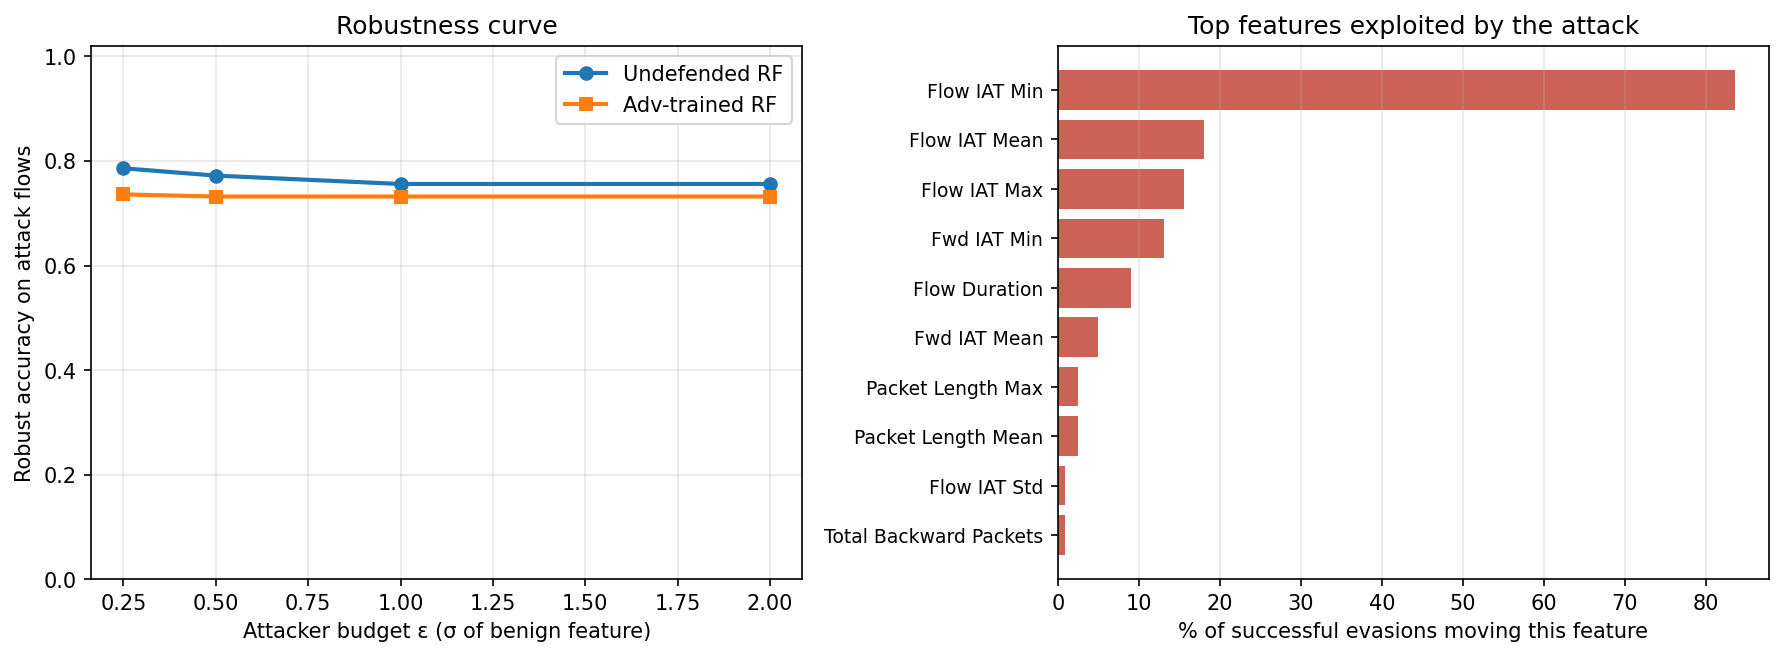
\includegraphics[width=0.85\textwidth]{adversarial_robustness.png}
    \caption{Robust accuracy as a function of perturbation budget
    $\varepsilon$ for the undefended and adversarially-trained random
    forests. Both curves flatten quickly; adversarial training shifts
    the curve downward (worse clean accuracy) without lifting it at
    large $\varepsilon$.}
    \label{fig:adv-robust}
\end{figure}

The successful evasions are concentrated in a small set of features:
Flow IAT Min is moved in 83.6\% of successful attacks, Flow IAT Mean in
18.0\%, Flow IAT Max in 15.6\%, Forward IAT Min in 13.1\%, and Flow
Duration in 9.0\%. Packet-length features are moved in fewer than 3\%
of attacks. This concentration suggests that rate limiting, traffic
shaping, or protocol-level constraints on inter-packet timing may
reduce the effectiveness of timing-based evasion, but validating this
in practice would require packet-level experiments outside this
thesis's scope.

The adversarial flows do not stay specific to the random forest that
generated them. When the same crafted flows are re-scored by XGBoost,
the transferability rate is 86.4\% --- almost the entire RF evasion set
fools XGBoost as well. By comparison, clean attack flows are
misclassified by XGBoost at only 26\%. The practical implication is
that an attacker need not know which model the defender deploys: an
attack crafted against random forest transfers to XGBoost nearly
perfectly, so a parallel-ensemble defence in which two models must
agree before alerting offers very little additional protection.

Following Madry et al.~\cite{Madry2018}, we attempted a naïve form of
adversarial training as a defence: 2{,}000 RF-adversarial attack flows
were added to the binary training set, the random forest was retrained,
and the threshold was retuned via Youden's J. The result is a clear
negative: clean F1 dropped from 0.859 to 0.734 (a 12.5-point loss) and
the evasion rate increased from 24.4\% to 26.8\%. The naïve defence
makes both clean and adversarial performance worse simultaneously. This
is consistent with the broader literature~\cite{Tramer2020}, which has
documented that off-the-shelf adversarial training without curriculum
scheduling, careful retuning, and data balancing often hurts both
metrics. Reporting the failure is informative: it demonstrates that
adversarial robustness for flow-based IDS is not solved by adding noise
to the training set.

The practical implication for a deployed flow-based IDS is concrete.
The 21.4\% bounded evasion rate and the 86.4\% cross-model
transferability together mean that two complementary controls are
needed: model-level monitoring (tracking evasion-shaped flows that sit
close to the decision boundary across multiple retraining cycles) and
network-level enforcement (rate limiting, traffic shaping, or
protocol-level inter-packet-timing constraints that shrink the
19-feature attacker-controllable subset). Neither is in scope here;
both follow naturally from the empirical findings.

\chapter{Best-Model Selection: Why Random Forest Wins for Deployment}
\label{ch:bestmodel}

The previous five chapters reported each evaluation in isolation. This
chapter aggregates the evidence and answers the practical question: if a
SOC could deploy only one of these four models tomorrow, which one
should it be?

Six criteria matter for a deployable IDS, in roughly this order of
importance: temporal stability (LODO mean and std), recall at
deployment-grade FPR budgets, calibration, inference latency,
adversarial robustness, and operational simplicity.

Table~\ref{tab:best-model} collapses every result in Part~III into a
single comparison. Each row is one criterion; each column is one model;
a star marks the best (or tied) model on that row. Random forest collects
six stars, XGBoost three, LightGBM two, and logistic regression two.

\begin{table}[H]
    \centering
    \caption{Cross-criterion comparison. $\star$ = best (or tied) on that row.}
    \label{tab:best-model}
    \footnotesize
    \begin{tabular}{lcccc}
        \toprule
        \textbf{Criterion} & \textbf{LogReg} & \textbf{Random Forest} & \textbf{XGBoost} & \textbf{LightGBM} \\
        \midrule
        Stratified multi-class macro F1 & 0.27 & 0.84 & \textbf{0.86 $\star$} & 0.30 \\
        Day-split multi-class macro F1 & 0.43 & 0.44 & 0.44 & \textbf{0.46 $\star$} \\
        Day-split binary F1 (Youden) & 0.68 & \textbf{0.86 $\star$} & 0.76 & 0.74 \\
        LODO mean ROC-AUC & 0.63 & \textbf{0.93 $\star$} & 0.92 & 0.84 \\
        LODO ROC-AUC std (lower=better) & 0.37 & \textbf{0.05 $\star$} & 0.09 & 0.21 \\
        Recall @ 0.1\% FPR (day binary) & 0.39 & \textbf{0.62 $\star$} & 0.03 & 0.46 \\
        Recall @ 1\% FPR (day binary) & 0.60 & \textbf{0.63 $\star$} & \textbf{0.64 $\star$} & 0.62 \\
        ECE (lower=better, day binary) & \textbf{0.07 $\star$} & 0.18 & 0.25 & 0.25 \\
        UNSW binary F1 & 0.89 & \textbf{0.92 $\star$} & \textbf{0.92 $\star$} & \textbf{0.92 $\star$} \\
        Latency $\mu$s/flow (bs=10k) & \textbf{0.11 $\star$} & 3.19 & 0.80 & 2.80 \\
        Adversarial evasion @ $0.25\sigma$ & n/a & 21.4\% & n/a & n/a \\
        \midrule
        \textbf{Total $\star$} & 2 & \textbf{6 $\star$} & 3 & 2 \\
        \bottomrule
    \end{tabular}
\end{table}

\interpretation{Random forest dominates the rows that matter most for
deployment: temporal stability, recall at strict FPR, and overall
ranking across LODO folds. It loses on stratified multi-class (XGBoost
wins) and on calibration (LogReg wins). For deployment, the wins it has
are the ones that matter.}

Random forest is the best deployment choice on three independent
grounds. \textbf{Temporal stability}: ROC-AUC $= 0.926 \pm 0.053$ across
LODO folds is the lowest standard deviation of any of the four models
(XGBoost $\pm 0.086$, LightGBM $\pm 0.212$, LogReg $\pm 0.374$).
Stability matters more than peak performance because production traffic
shifts continuously. \textbf{Operational sweet spot at strict FPR}: at
0.1\% FPR the random forest catches 62\% of attacks, while XGBoost
catches 3\%, LightGBM catches 46\%, and logistic regression catches
39\%. \textbf{Reasonable speed and simplicity}: random forest is the
slowest of the four at 3.2~$\mu$s/flow, but still 200 times faster than
the throughput a saturated 1~Gbps mirror tap produces. Its single-step
training and native parallel evaluation make it operationally simpler
than gradient-boosting alternatives.

Three caveats apply. Multi-class on the day split is hard for random
forest just as for the other tree ensembles --- all three reach macro F1
of approximately 0.44 because of the unseen-class problem. Calibration
on the day split is poor (ECE 0.18 versus LogReg's 0.07), and any
deployment that exposes probability scores to downstream tooling should
apply Platt scaling or isotonic regression as post-processing. Finally,
adversarial robustness is shared with the other tree models: the 21.4\%
evasion rate at $\varepsilon = 0.25\sigma$ (or 24.4\% if the attacker is
allowed to run unbounded) is not made better by choosing random forest
over XGBoost or LightGBM, and network-layer mitigations (rate limiting,
traffic shaping, or protocol-level constraints on inter-packet timing)
are needed in addition to the model itself; their effectiveness would
need packet-level validation outside this thesis's scope.

The deployment recommendation: random forest as the binary detector
with Youden-J threshold tuning per fold, retrained weekly on a rolling
four-week window. Keep XGBoost as a transferability sanity check rather
than as a defence: adversarial flows that evade random forest transfer
to XGBoost at 86\%, so the two models do not catch independent failure
modes, but a divergence between them on a particular flow is a useful
out-of-distribution signal. Reserve LightGBM for UNSW-style multi-class
tasks where it leads. Use logistic regression as the calibration
baseline.


\thesispart{Practice}
\chapter{Operational Triage: OODA Loop and MITRE ATT\&CK Mapping}
\label{ch:mitre}

A machine-learning intrusion detector does not run in isolation. It
feeds into a SOC staffed by human analysts, integrates with a SIEM, and
is ultimately judged on whether it helps the organisation respond to
real incidents. This chapter sketches how the artefacts produced by
this thesis fit into a SOC workflow, organised by Boyd's OODA loop, and
documents the MITRE ATT\&CK mapping that turns model output into
playbook-ready alerts.

\section{The OODA Loop in a SOC Workflow}

Boyd's OODA loop --- Observe, Orient, Decide, Act --- describes the
decision cycle of any adversarial engagement. Whoever cycles faster
wins. In a SOC context, ``Observe'' is alert ingestion, ``Orient'' is
enrichment with context (reputation lookups, asset criticality, MITRE
mapping), ``Decide'' is the analyst's classification of the alert as a
real incident or a false positive, and ``Act'' is containment and
remediation.

In this thesis, the trained binary detector lives at the Observe stage:
the flow extractor ingests packets, the model scores each flow, and an
alert is emitted when the predicted probability exceeds the Youden-J
threshold. Inference latency at batch~=~10{,}000 is 3.2~$\mu$s/flow for
random forest --- well under any operational requirement. The MITRE
mapping described in Section~\ref{sec:mitre-mapping} provides the Orient
enrichment that turns the alert from ``probability 0.97'' into a
structured story: ``FTP-Patator on port 21, T1110.001 Brute Force,
Credential Access, from external IP X with 1{,}400 similar alerts in the
last hour''.

The analyst's Decide step --- escalate or close --- shrinks under this
enrichment because the alert routes directly to a known playbook (T1110
to credential-stuffing playbook; T1498 to DDoS playbook). The detector
itself does not Act; it produces evidence for action, which is taken by
humans or by automation rules tied to playbook outcomes. This separation
is intentional: a detector with a 21\%--24\% adversarial evasion rate
cannot be trusted to make blocking decisions autonomously.

The bottleneck in OODA is the analyst's Decide step (microseconds for
the detector, sub-second for the orchestrator, minutes for the human).
The MITRE mapping is therefore the single largest force multiplier in
this design, because it removes the manual ``which playbook applies''
step.

\section{Mapping Predictions to MITRE ATT\&CK}
\label{sec:mitre-mapping}

MITRE ATT\&CK~\cite{Strom2018} is the industry-standard taxonomy for
adversary behaviour, organised by tactic (the ``why'') and technique
(the ``how''). It is more granular than the Lockheed kill chain (over
200 techniques) and is maintained as an open knowledge base. SOC
playbooks are usually keyed to ATT\&CK technique IDs, so mapping
classifier output to ATT\&CK lets the SOC route alerts to existing
playbooks rather than triaging each prediction in isolation.

\begin{figure}[H]
    \centering
    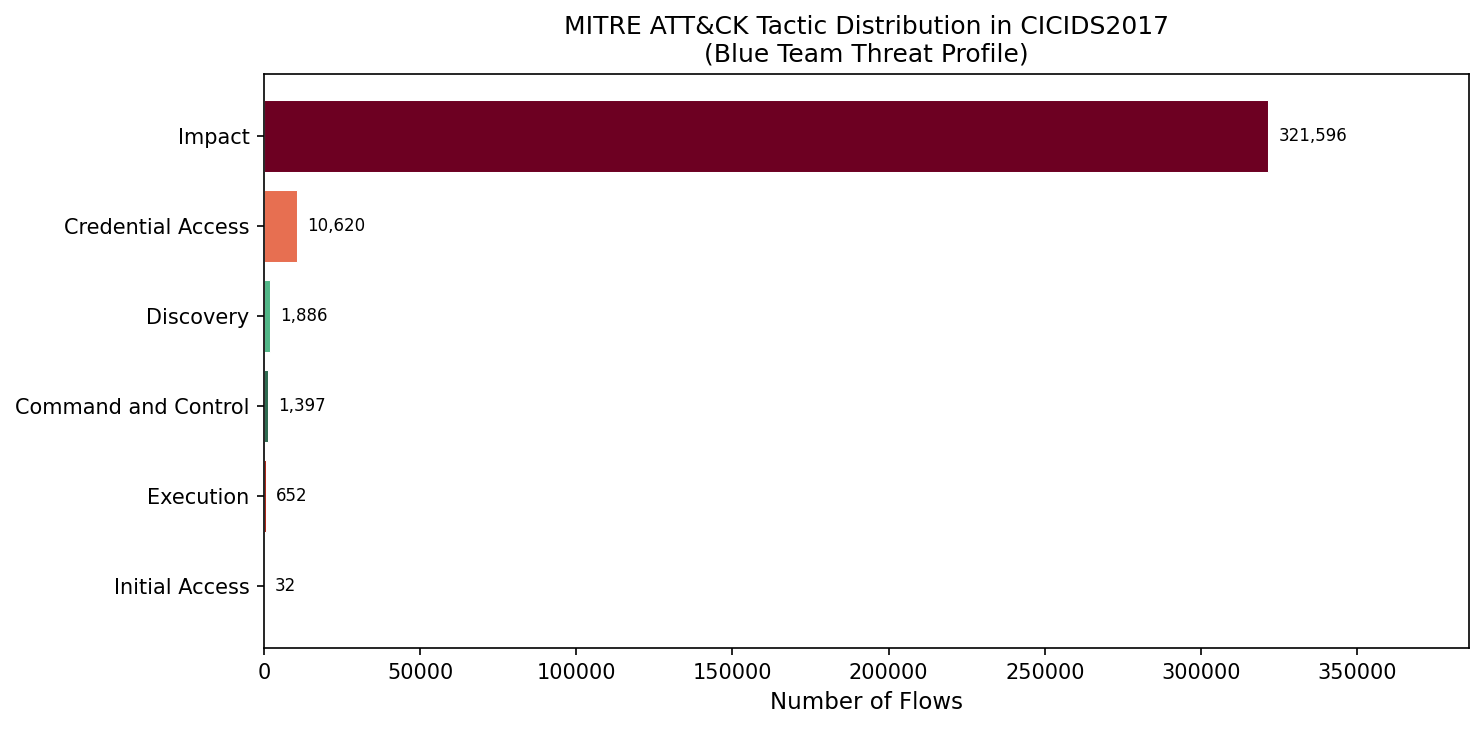
\includegraphics[width=0.85\textwidth]{tactic_distribution.png}
    \caption{Distribution of CICIDS2017 attack flows across MITRE ATT\&CK
    tactics. The dataset is dominated by Impact (DDoS, DoS Hulk) and
    Credential Access (Patator) tactics; Initial Access techniques such
    as Heartbleed contribute very few flows.}
    \label{fig:tactic-distribution}
\end{figure}

The binary random-forest detector produces high-precision alerts on
T1498 (Network Denial of Service: DDoS and DoS Hulk) and T1046 (Network
Service Discovery: PortScan). These attack types have distinctive flow
signatures --- short, bursty, asymmetric for DoS; many short flows to
many ports for PortScan --- and the detector catches them at low FPR
with high precision.

Multi-class predictions on the day split are unusable for sub-class
attribution because the model cannot output a label it has not seen.
Heartbleed (T1190) has only 11 examples in the dataset; Web Attack
subtypes are confused with each other. The deployed system therefore
uses the binary head to flag, and the multi-class head only when the
predicted class is in-distribution.

\begin{table}[H]
    \centering
    \caption{Predicted class to MITRE ATT\&CK mapping.}
    \label{tab:mitre-mapping}
    \footnotesize
    \begin{tabular}{p{4.0cm}p{1.8cm}p{5.0cm}p{3.5cm}}
        \toprule
        \textbf{Predicted class} & \textbf{ATT\&CK ID} & \textbf{Technique} & \textbf{Phase} \\
        \midrule
        FTP-Patator & T1110.001 & Brute Force: Password Guessing & Credential Access \\
        SSH-Patator & T1110.001 & Brute Force: Password Guessing & Credential Access \\
        Web Attack-Brute Force & T1110 & Brute Force & Credential Access \\
        DDoS & T1498 & Network Denial of Service & Impact \\
        DoS Hulk / GoldenEye & T1498 & Network Denial of Service & Impact \\
        DoS Slowhttptest / slowloris & T1499 & Endpoint Denial of Service & Impact \\
        PortScan / Infiltration & T1046 & Network Service Discovery & Discovery \\
        Bot & T1071.001 & Application Layer Protocol: Web Protocols & Command and Control \\
        Heartbleed / SQLi & T1190 & Exploit Public-Facing Application & Initial Access \\
        Web Attack-XSS & T1059.007 & Command and Scripting: JavaScript & Execution \\
        \bottomrule
    \end{tabular}
\end{table}

The mapping is static for two reasons. First, a learned mapping would
require richer telemetry than this thesis has access to (logs, EDR,
identity signals). Second, the static mapping is auditable and portable:
a successor SOC can read the JSON file, understand exactly why a given
prediction routes to a given playbook, and modify the mapping if their
attack catalogue or playbook taxonomy differs.

\chapter{Deployment Considerations}
\label{ch:deployment}

This chapter collects two deployment-related findings: inference latency
under expected throughput, and an honest comparison against unsupervised
anomaly-detection baselines.

\section{Inference Latency and Throughput}

Inference latency is not the bottleneck for any of the four models. At
batch~=~10{,}000 (a typical NIDS collector burst size), per-flow latency
is 0.11~$\mu$s for logistic regression, 0.80~$\mu$s for XGBoost,
2.80~$\mu$s for LightGBM, and 3.19~$\mu$s for random forest. A
saturated 1~Gbps mirror tap produces approximately 1{,}700 flows per
second --- two orders of magnitude below even the slowest model's
throughput of 313{,}400 flows per second.

\begin{table}[H]
    \centering
    \caption{Per-flow inference latency at batch=10{,}000 on the binary day split.}
    \label{tab:latency}
    \small
    \begin{tabular}{lcc}
        \toprule
        \textbf{Model} & \textbf{$\mu$s / flow (bs=10k)} & \textbf{Flows / second} \\
        \midrule
        LogReg & 0.11 & 9{,}108{,}090 \\
        XGBoost & 0.80 & 1{,}248{,}123 \\
        LightGBM & 2.80 & 356{,}793 \\
        Random Forest & 3.19 & 313{,}400 \\
        \bottomrule
    \end{tabular}
\end{table}

Model selection should therefore be driven by accuracy, robustness, and
operational simplicity, not by latency. Any of the four models can keep
up with a typical enterprise mirror tap on a single CPU core; latency
becomes a factor only at much higher throughputs (saturated 100~Gbps
backbones), which are out of scope here.

\section{Unsupervised Anomaly Detection as an Honest Baseline}

A natural question is whether the labels are doing real work --- could
the same detection performance be achieved without them? To answer, two
unsupervised baselines were trained on Monday-to-Wednesday benign flows
only: Isolation Forest and Local Outlier Factor (LOF). Both flag Friday
anomalies without ever having seen a labelled attack.

Isolation Forest reaches ROC-AUC $= 0.807$ on the binary day task; LOF
reaches $0.849$. Both are substantially worse than the supervised
random forest at ROC-AUC $= 0.940$, which confirms that the attack
labels carry real signal. The gap widens at strict FPR budgets: at 1\%
FPR, Isolation Forest catches only about 1\% of attacks while the
supervised random forest catches 63\%. Unsupervised detection is not
bad in the abstract --- it works without labels, which is valuable ---
but at the FPR budgets where a real SOC operates, supervised wins
decisively. The practical recommendation is to use unsupervised
detection as a novelty layer alongside the supervised detector for
known attack families, rather than as a replacement.


\thesispart{Closing}
\chapter{Discussion and Limitations}
\label{ch:discussion}

\section{What Worked}

Binary detection on the day split survives temporal shift better than
prior expectations. Random forest at F1 = 0.86 with a 6.5\% FPR is the
deployment-relevant ballpark for organisations that can absorb a
moderate alert budget --- though production deployment requires
live-traffic validation, drift monitoring, and the network-layer
mitigations discussed in Chapter~\ref{ch:adversarial}. The LODO study
gave a stronger generalisation claim than any single split: ROC-AUC =
$0.926 \pm 0.053$ across days with very different attack mixes is a
narrow band that survives genuinely disjoint test scenarios. The MITRE
ATT\&CK mapping turns probability scores into operational alerts. The
reproducible pipeline (45--60 minutes, single Makefile target) is a
real artefact a successor researcher can extend.

\paragraph{Engineering maturity.}
Three small engineering choices accumulated into the most useful
property of this work: a deterministic \texttt{random\_state}, a single
Makefile entry point that runs the whole pipeline end to end, and an
explicit leakage-check module that fails loudly if the four rate
features are reintroduced. None of these are research contributions ---
they are the difference between a thesis a successor researcher can
extend in an afternoon and one they have to rebuild from scratch.

\section{What Did Not Work}

Multi-class classification on the day split. Naïve adversarial training.
Both negative results are informative: the first establishes a hard
structural limit (the model cannot output a label that does not exist in
training), the second establishes that off-the-shelf defences fail. The
adversarial-training failure is consistent with Tramer et
al.~\cite{Tramer2020}, who documented similar failures across many
adversarial-training schemes. Reporting these failures rather than
hiding them is part of the contribution: a successor researcher knows
what not to waste time on. The naïve defence dropped clean F1 from
0.859 to 0.734 and increased evasion from 24.4\% to 26.8\% --- the
worst possible outcome for a defence.

Three findings during the experimental phase surprised the author and
are worth recording. The most concentrated adversarial brittleness:
83.6\% of successful evasions move a single feature, Flow IAT Min. The
narrow LODO ROC-AUC variance for random forest at $\pm 0.053$ across
genuinely disjoint test scenarios. And the sharp rank reversal between
CICIDS and UNSW datasets: the CICIDS-best model is not the UNSW-best.
Headline benchmark numbers measure the dataset they were generated on at
least as much as they measure the quality of the model.

\section{Threats to Validity}

\paragraph{Dataset limitations.} Both CICIDS2017 and UNSW-NB15 are
synthetic captures from controlled testbeds. Real enterprise traffic is
messier: more diverse user behaviour, more encrypted (TLS) traffic, a
long-tailed distribution of rare attack variants. Numbers obtained on
synthetic data are likely upper bounds on what would be achievable in
production. CICIDS2017 also has documented labelling
errors~\cite{Engelen2021} which we did not relabel.

\paragraph{Evaluation limitations.} LODO is over a single dataset;
cross-dataset LODO would be stronger. Multi-threaded non-determinism
introduces approximately 1\% F1 drift between runs. McNemar's test
assumes independent samples; flows in CICIDS share temporal
correlations, so the McNemar $p$-values reported in
Section~\ref{sec:mcnemar} should be read as supporting evidence for the
model ranking rather than as exact significance levels.

\paragraph{Attacker-model limitations.} The threat model assumes
score-query black-box access with unlimited queries; many real
deployments rate-limit query access, which slows but does not change the
qualitative outcome. The $L^\infty$ budget on a 19-feature subset is a
simplification. Most importantly, the thesis perturbs feature vectors
rather than synthesising adversarial network packets. Bridging the
problem-space gap (Pierazzi et al.~\cite{Pierazzi2020}) is open work.

\paragraph{Deployment limitations.} The MITRE mapping is a static JSON
file rather than a learned mapping over richer telemetry. There is no
streaming or online mode. There is no adversary simulator: we assume
the attacker is greedy and uses a fixed budget, while a sophisticated
real attacker would adapt their strategy based on observed detector
behaviour.

\section{Relation to the Published Literature}

The thesis sits in a small but growing literature on honest evaluation
of ML-based intrusion detection. Engelen et al.~\cite{Engelen2021}
flagged the leakage rate features in CICIDS2017 --- we replicate the
finding and drop those columns explicitly, confirming the
four-percentage-point effect on stratified RF macro F1. Sharafaldin et
al.~\cite{Sharafaldin2018} reported macro F1 $\approx 0.97$ on CICIDS
using stratified splits; we reproduce 0.86 (XGBoost) on the same
protocol after leakage filtering, and 0.44 on the day split. Apruzzese
et al.~\cite{Apruzzese2019} demonstrated adversarial brittleness for
flow-based IDS classifiers; the 21.4\% bounded evasion rate
(24.4\% unbounded headline) reported here is in the same ballpark, with
the additional finding that the brittleness is concentrated in a single
feature. The pattern across the references is consistent: the attack
side of the literature is mature, and the defence side has many more
unsolved problems than solved ones.

\chapter{Conclusion and Future Work}
\label{ch:conclusion}

\section{Answers to the Research Questions}

\paragraph{RQ1 -- Does flow-based ML generalise across time?}
The answer depends on the task formulation. Multi-class classification
does not generalise: macro F1 collapses from 0.86 on the random
stratified split to 0.44 on the day-based temporal split, with all four
models within 0.04 of one another. The collapse is structural --- Friday's
classes are not in training --- and model tuning cannot recover the loss.
Binary detection, however, does largely generalise: random forest reaches
F1 = 0.86 on the day split and ROC-AUC = $0.926 \pm 0.053$ across
leave-one-day-out folds.

\paragraph{RQ2 -- Are flow-based detectors robust to low-effort evasion?}
No. The undefended random forest flips 21.4\% of attack flows at
$\varepsilon = 0.25\sigma$ on the perturbable feature subset, with a
looser headline evasion rate of 24.4\% when the attack is run unbounded,
and 83.6\% of successful evasions move a single feature (Flow IAT Min).
Adversarial flows transfer to XGBoost at 86.4\%, so ensemble-based
defences are ineffective against this kind of attack. Naïve adversarial
training fails: clean F1 drops from 0.86 to 0.73 while evasion increases
to 26.8\%.

\paragraph{RQ3 -- Can model output drive triage?}
Yes, via static MITRE ATT\&CK mapping. The pipeline produces structured
per-flow alerts annotated with technique ID, kill-chain phase, and a
one-sentence justification, ready for direct routing to SOC playbooks.
Sub-class attribution on the day split is unreliable for the same
structural reason that drives the multi-class collapse, so the deployed
system defaults to ``unspecified attack'' when the multi-class prediction
is out-of-distribution.

\section{Future Work}

Five directions stand out. First, cross-dataset LODO --- training on
CICIDS days and testing on UNSW splits --- would extend the temporal
generalisation claim across capture environments. Second, the static
MITRE mapping could be replaced with a learned mapping using richer
telemetry. Third, a stronger adversarial training defence (PGD with
curriculum scheduling, balanced augmentation, classifier-rebalanced
thresholds) would test whether the negative result on naïve adversarial
training can be overturned with a more careful approach. Fourth,
streaming evaluation --- deploying as a Kafka consumer with continuous
concept-drift detection --- would test the deployment artefacts under
realistic operational load. Fifth, modern tabular and sequence models
(TabNet, FT-Transformer, LSTM-over-IATs) deserve a careful comparison
against the tree-ensemble baseline.

\section{Closing Statement}

Flow-based machine learning for intrusion detection works in practice,
but only when it is evaluated under protocols that respect the temporal
structure of the data. On the two benchmarks studied here, headline
numbers from random stratified splits substantially overstate the
deployment-relevant performance reported under day-based and LODO
splits. Binary detection is the more credible deployment framing on
these benchmarks, MITRE-mapped triage is operationally valuable, and
the entire pipeline is reproducible in 45 to 60 minutes on a laptop.
The integration --- honest temporal evaluation, adversarial robustness,
and operational MITRE triage in one reproducible pipeline --- is what
distinguishes this thesis from a benchmark replay. The unsolved problem
is adversarial robustness: any deployed detector should assume that a
determined adversary will eventually evade it, and the right response is
to combine the machine-learning detector with network-layer mitigations,
host-based detection, and human analysts in a defence-in-depth
architecture.


\printbibliography[title={Bibliography}]
\addcontentsline{toc}{chapter}{Bibliography}

\appendix
\chapter{Full Hyperparameter Specification}
\label{app:hyperparams}

\begin{table}[H]
    \centering
    \caption{Full hyperparameter specification.}
    \label{tab:hyperparams}
    \footnotesize
    \begin{tabular}{p{4.0cm}p{10.5cm}}
        \toprule
        \textbf{Model / Setting} & \textbf{Configuration} \\
        \midrule
        Random Forest (multi-class) & \texttt{n\_estimators=300, max\_depth=24, max\_features='sqrt', class\_weight='balanced\_subsample', random\_state=42, n\_jobs=-1} \\
        \addlinespace
        Random Forest (binary) & \texttt{n\_estimators=300, max\_depth=24, max\_features='sqrt', class\_weight='balanced\_subsample', random\_state=42, n\_jobs=-1} \\
        \addlinespace
        XGBoost (multi-class) & \texttt{n\_estimators=200, max\_depth=8, learning\_rate=0.1, subsample=0.9, colsample\_bytree=0.9, eval\_metric='mlogloss'} \\
        \addlinespace
        XGBoost (binary) & \texttt{n\_estimators=400, max\_depth=8, learning\_rate=0.05, subsample=0.9, colsample\_bytree=0.9, scale\_pos\_weight=neg/pos} \\
        \addlinespace
        LightGBM (multi-class) & \texttt{n\_estimators=200, max\_depth=8, learning\_rate=0.1, num\_leaves=63, min\_child\_samples=20} \\
        \addlinespace
        LightGBM (binary) & \texttt{n\_estimators=400, max\_depth=8, learning\_rate=0.05, num\_leaves=63, min\_child\_samples=20, is\_unbalance=True} \\
        \addlinespace
        Logistic Regression & \texttt{solver='saga', max\_iter=2000, tol=1e-3, C=1.0, class\_weight='balanced'}, with a \texttt{StandardScaler} pipeline \\
        \addlinespace
        Threshold method & Youden's J on validation set, all binary models \\
        \addlinespace
        Adversarial attack & Greedy coordinate-ascent, 15 iterations, 6 step magnitudes per feature, $L^\infty$ in $\sigma$ units, perturbable subset = 19/73 \\
        \addlinespace
        Adversarial training & 2{,}000 RF-adversarial flows added to binary training set, RF retrained, threshold retuned via Youden's J \\
        \addlinespace
        Bootstrap CIs & $B = 1000$ percentile resamples, seed = 42 \\
        \addlinespace
        Random seed & \texttt{random\_state = 42} throughout (see \texttt{config.RNG}); approximately 1\% F1 drift between runs from multi-threaded tree ensembles \\
        \bottomrule
    \end{tabular}
\end{table}

\chapter{Reproducibility}
\label{app:reproducibility}

Every numerical result can be reproduced from the original CSV downloads
in approximately 45--60 minutes on a 2024 MacBook Pro M-series:

\begin{verbatim}
git clone <repository URL>
cd bsc-thesis-ids
python -m venv .venv && source .venv/bin/activate
pip install -r requirements.txt
# Place CICIDS2017 CSVs in data/raw/cicids2017/
# Place UNSW-NB15 CSVs in data/unsw-nb15/raw/
caffeinate -i make full     # macOS; on Linux use systemd-inhibit
\end{verbatim}

The \texttt{make full} target chains every step of the pipeline: data
preparation, sanity checks, training under both split policies, binary
training, evaluation, LODO cross-validation, UNSW training and
evaluation, MITRE mapping, traffic analysis, figure generation,
inference benchmarking, bootstrap confidence intervals, operating
points, anomaly detection, and adversarial evaluation. Individual
targets can be run in isolation.

The random seed is set to 42 throughout. Tree ensembles trained with
\texttt{n\_jobs=-1} introduce approximately 1\% F1 drift between runs
because of non-deterministic thread scheduling at leaf-split time.
Numbers in this thesis come from a single canonical run validated
against a second run to confirm the qualitative conclusions hold under
the drift.

\paragraph{Near-duplicate filtering sensitivity.}
A sensitivity study confirms that macro F1 on the binary day task
changes by less than 0.01 across all four models when near-duplicates
are filtered. This result should be read alongside the leakage-check
report, which flags many near-duplicate groups that cross the
train/test boundary in both stratified and day splits. Exact duplicates
are removed in cleaning; near-duplicates that survive are mostly
within-class neighbours (similar attack flows from the same campaign)
rather than benign-versus-attack confusables, so they do not materially
shift macro F1 on the binary task. A stricter near-duplicate pruning
would likely change per-class precision/recall and is the kind of
signal that Pendlebury et al.~\cite{Pendlebury2019} argue should be
reported explicitly rather than averaged away.

\begin{figure}[H]
    \centering
    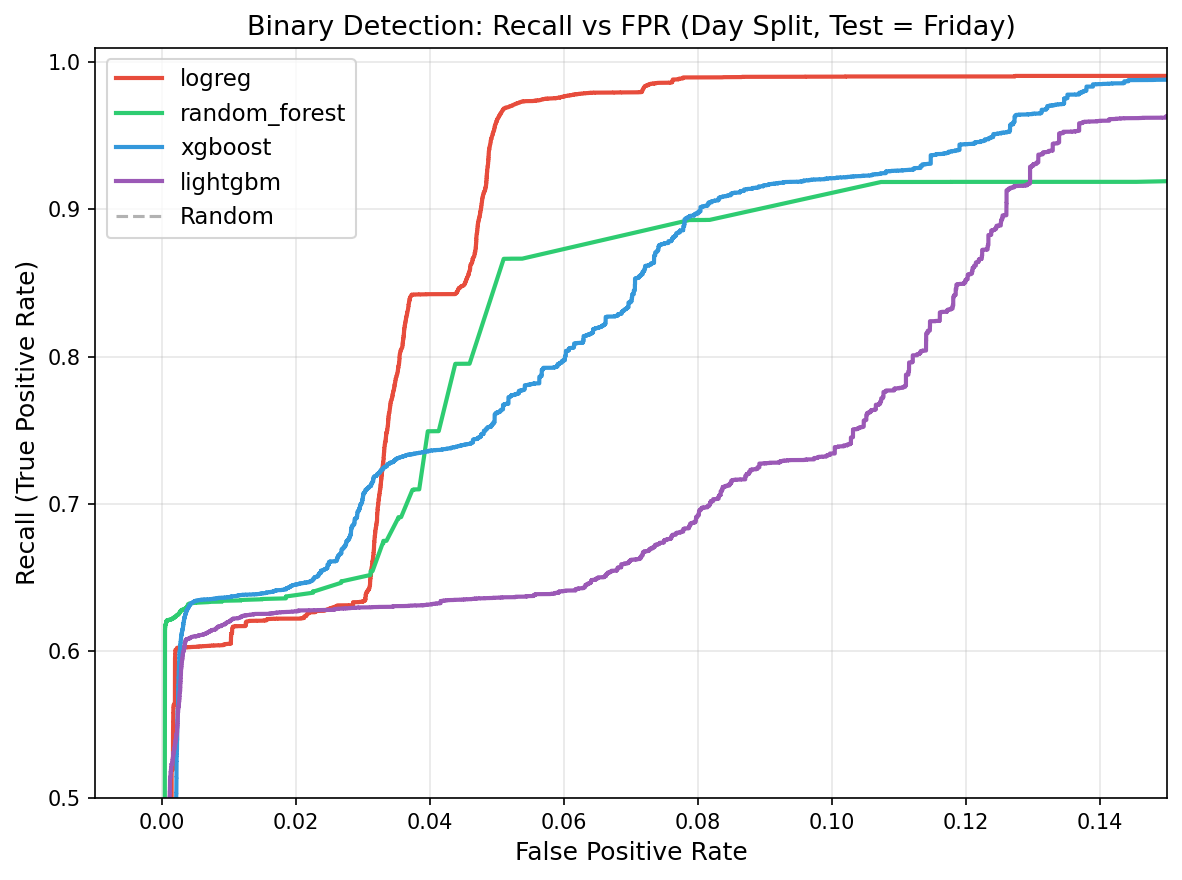
\includegraphics[width=0.8\textwidth]{figure_V3_binary_recall_vs_fpr.png}
    \caption{Recall-versus-FPR sweep for all four binary models on the
    day test set. The full operating-point curve from which the headline
    operating points in Table~\ref{tab:operating-points} are drawn.}
    \label{fig:v3}
\end{figure}

\chapter{Glossary of Terms}
\label{app:glossary}

Plain-English definitions for security-specific terms used in this
thesis. Standard machine-learning terminology (precision, recall, ROC,
ETC.) is in the List of Abbreviations.

\begin{longtable}{p{4.0cm}p{11.0cm}}
    \toprule
    \textbf{Term} & \textbf{Definition} \\
    \midrule
    \endfirsthead
    \toprule
    \textbf{Term} & \textbf{Definition} \\
    \midrule
    \endhead
    Adversarial example & An input crafted to fool a machine-learning model into the wrong prediction. \\
    Adversarial training & Training a model on a mix of clean and adversarial examples to make it more robust. \\
    Anomaly detection & Detecting traffic that deviates from a learned baseline of normal behaviour. \\
    Bootstrap & A resampling-based statistical technique for estimating uncertainty. \\
    Brute force & Repeated guessing of credentials or keys until access is gained. \\
    Calibration & How closely a model's predicted probabilities match real-world frequencies. \\
    Concept drift & When the statistical properties of input data change over time. \\
    Day-split & Train on early days, test on later days; respects temporal order. \\
    DDoS & Distributed Denial of Service --- many sources flooding a target. \\
    EDR & Endpoint Detection and Response --- security software on every host. \\
    Evasion attack & An adversarial attack that flips a true positive to a false negative. \\
    Flow & A sequence of packets sharing source/destination IP, ports, and protocol. \\
    Heartbleed & A 2014 OpenSSL vulnerability that leaked memory contents. \\
    Kill chain & Lockheed Martin's seven-stage model of a typical intrusion. \\
    Leakage & When information from the test set inadvertently informs training. \\
    LODO & Leave-One-Day-Out --- train on $n - 1$ days, test on the held-out day. \\
    $L^\infty$ norm & The largest absolute change across all dimensions; bounds adversarial budgets. \\
    McNemar's test & A statistical test for comparing two classifiers on the same test set. \\
    MITRE ATT\&CK & An open framework cataloguing real-world attacker techniques. \\
    OODA loop & Boyd's Observe-Orient-Decide-Act decision cycle. \\
    Operating point & A specific threshold choice on the precision-recall trade-off curve. \\
    SHAP & A method for attributing a model's prediction to its input features. \\
    SIEM & Security Information and Event Management --- central alert aggregator. \\
    SOAR & Security Orchestration, Automation, and Response --- the playbook engine. \\
    SOC & Security Operations Centre --- the team that watches the network. \\
    Stratified split & A random split that preserves class proportions in every partition. \\
    Threat model & A formal description of who the attacker is and what they can do. \\
    Transferability & An adversarial example crafted against one model fooling another. \\
    Youden's J & TPR $-$ FPR; a prevalence-invariant threshold-selection criterion. \\
    \bottomrule
\end{longtable}


\end{document}
